% !TeX spellcheck = ru_RU
\newif\ifanswers

\documentclass[aspectratio=169
  , xcolor={svgnames}
  , hyperref=
      { colorlinks
      , urlcolor=DarkBlue 
      }  
  , russian  % This line affects translation of theorem titles
  ]{beamer}

\makeatletter
\@ifclassloaded{beamer}{
  % get rid of header navigation bar
  \setbeamertemplate{headline}{}
  % get rid of bottom navigation symbols
  \setbeamertemplate{navigation symbols}{}
  % get rid of footer
  %\setbeamertemplate{footline}{}
}
{}
\makeatother
%%%%%%%%%%%%%%%%%%%%%%%%%%%%%%%%%%%%%%%%%%%%%
\usepackage{fontawesome}
% \newfontfamily{\FA}{Font Awesome 5 Free} % some glyphs missing
\expandafter\def\csname faicon@facebook\endcsname{{\FA\symbol{"F09A}}}
\def\faQuestionSign{{\FA\symbol{"F059}}}
\def\faQuestion{{\FA\symbol{"F128}}}
\def\faExclamation{{\FA\symbol{"F12A}}}
\def\faUploadAlt{{\FA\symbol{"F093}}}
\def\faLemon{{\FA\symbol{"F094}}}
\def\faPhone{{\FA\symbol{"F095}}}
\def\faCheckEmpty{{\FA\symbol{"F096}}}
\def\faBookmarkEmpty{{\FA\symbol{"F097}}}

\newcommand{\faGood}{\textcolor{ForestGreen}{\faThumbsUp}}
\newcommand{\faBad}{\textcolor{red}{\faThumbsODown}}
\newcommand{\faWrong}{\textcolor{red}{\faTimes}}
\newcommand{\faMaybe}{\textcolor{blue}{\faQuestion}}
\newcommand{\faCheckGreen}{\textcolor{ForestGreen}{\faCheck}}
%%%%%%%%%%%%%%%%%%%%%%%%%%%%%%%%%%%%%%%%%%%%%

\usepackage{fontspec}
\usepackage{xunicode}
\usepackage{xltxtra}
\usepackage{xecyr}
\usepackage{hyperref}

\setmainfont[
 Ligatures=TeX,
 Extension=.otf,
 BoldFont=cmunbx,
 ItalicFont=cmunti,
 BoldItalicFont=cmunbi,
% Scale = 1.1
]{cmunrm}
\setsansfont[
 Ligatures=TeX,
 Extension=.otf,
 BoldFont=cmunsx,
 ItalicFont=cmunsi,
%  Scale = 1.2
]{cmunss}
%\setmainfont[Mapping=tex-text]{DejaVu Serif}
%\setsansfont[Mapping=tex-text]{DejaVu Sans}
%\setmonofont{Fira Code}[Contextuals=AlternateOff]
\setmonofont{Fira Code}[Contextuals=Alternate,Scale=0.9]
\newfontfamily{\myfiracode}[Scale=1.5,Contextuals=Alternate]{Fira Code}
%\setmonofont[Scale=0.9,BoldFont={Inconsolata Bold}]{Inconsolata}

\usepackage{polyglossia}
\setmainlanguage{russian}
\setotherlanguage{english}


%\newfontfamily\dejaVuSansMono{DejaVu Sans Mono}
% https://github.com/vjpr/monaco-bold/raw/master/MonacoB/MonacoB.otf
%\newfontfamily\monacoB{MonacoB}
%%%%%%%%%%%%%%%%%%%%%%%%%%%%%%%%%%%%%%%%%%%%%%%5
\usepackage{soul} % for \st that strikes through
\usepackage[normalem]{ulem} % \sout

\usepackage{stmaryrd}
\newcommand{\sem}[1]{\ensuremath{\llbracket #1\rrbracket}}


\usepackage{listings}
%\lstdefinestyle{style1}{
%  language=haskell,
%  numbers=left,
%  stepnumber=1,
%  numbersep=10pt,
%  tabsize=4,
%  showspaces=false,
%  showstringspaces=false
%}
%\lstdefinestyle{hsstyle1}
%{ language=haskell
%%          , basicstyle=\monacoB
%         , deletekeywords={Int,Float,String,List,Void}
%         , breaklines=true
%         , columns=fullflexible
%         , commentstyle=\color{ForestGreen}
%         , escapeinside=§§
%         , escapebegin=\begin{russian}\commentfont
%         , escapeend=\end{russian}
%         , commentstyle=\color{ForestGreen}
%         , escapeinside=§§
%         , escapebegin=\begin{russian}\color{ForestGreen}
%         , escapeend=\end{russian}
%         , mathescape=true
%%          , backgroundcolor = \color{MyBackground}
%}
%
%\newcommand{\inline}[1]{\lstinline{haskell}{#1}}
%\def\hsinline{\mintinline{haskell}}
%\def\inline{\hsinline}
%
%\lstnewenvironment{hslisting} {
%    \lstset { style={hsstyle1} }
%  }
%  {}
%  
%%%%%%%%%%%%%%%%%%%%%%%%%%%%%%%%%%%%%%%%%%%%%%%%%%%%%%%%%%%  
%%\setmainfont[
%% Ligatures=TeX,
%% Extension=.otf,
%% BoldFont=cmunbx,
%% ItalicFont=cmunti,
%% BoldItalicFont=cmunbi,
%%]{cmunrm}
%%% С засечками (для заголовков)
%%\setsansfont[
%% Ligatures=TeX,
%% Extension=.otf,
%% BoldFont=cmunsx,
%% ItalicFont=cmunsi,
%%]{cmunss}
%% \setmonofont[Scale=0.6]{Monaco}
%
%\usefonttheme{professionalfonts}
%\usepackage{times}
\usepackage{tikz}
\usetikzlibrary{cd}
\usepackage{tikz-cd}
\usepackage{caption}
\usepackage{subcaption}

%\renewtheorem{definition}{برهان}[chapter]
%%\DeclareMathOperator{->}{\rightarrow}
%\newcommand\iso{\ensuremath{\cong}}
%\usepackage{verbatim}
%\usepackage{graphicx}
%\usetikzlibrary{arrows,shapes}

%\usepackage{amsmath}
%\usepackage{amsfonts}
\usepackage{scalerel}
\DeclareMathOperator*{\myvee}{\scalerel*{\vee}{\sum}}
\DeclareMathOperator*{\mywedge}{\scalerel*{\wedge}{\sum}}

%
%\usepackage{tabulary}
%
%% sudo aptget install ttf-mscorefonts-installer
%%\setmainfont{Times New Roman}
%%\setsansfont[Mapping=tex-text]{DejaVu Sans}
%
%%\setmonofont[Scale=1.0,
%%    BoldFont=lmmonolt10-bold.otf,
%%    ItalicFont=lmmono10-italic.otf,
%%    BoldItalicFont=lmmonoproplt10-boldoblique.otf
%%]{lmmono9-regular.otf}
%
\usepackage[cache=true]{minted}
\usemintedstyle{perldoc}

\def\hsinline{\mintinline{haskell}}
\def\mlinline{\mintinline{ocaml}}
% color options
\definecolor{YellowGreen} {HTML}{B5C28C}
\definecolor{ForestGreen} {HTML}{009B55}
\definecolor{MyBackground}{HTML}{F0EDAA}



\institute{матмех СПбГУ}

\addtobeamertemplate{title page}{}{
  \begin{center}{\tiny Дата сборки: \today}\end{center}
}

\usepackage{tabulary}
\usepackage{verbatim}

\newcommand{\term}[2]{\textit{#1} (#2)}

\usepackage{amsthm}
\newtheorem{remark}{\textbf{Замечание}}[section]
\newtheorem{notation}{\textbf{Нотация}}[section]
\newtheorem{idea}{\textbf{Идея}}
\newtheorem{hint}{\textbf{Указание разработчикам}}[section]

\newtheoremstyle{exerciseStyle1}
{}                % Space above
{}                % Space below
{}                % Theorem body font % (default is "\upshape")
{}                % Indent amount
{\bfseries}       % Theorem head font % (default is \mdseries)
{.}               % Punctuation after theorem head % default: no punctuation
{ }               % Space after theorem head
{}                % Theorem head spec
\theoremstyle{exerciseStyle1}
\newtheorem{exercise}{\textbf{Упражнение}}[section]


\deftranslation[to=russian]{Theorem}{Теорема}
\deftranslation[to=russian]{theorem}{теорема}

\usepackage{tikz}
\usetikzlibrary{trees,decorations.pathreplacing}

\usepackage{subcaption}

%%%%%%%%%%%%%%%%%%
\makeatletter
\newenvironment{tabminted}{
  \let\FV@ListVSpace\relax
  \minted
}{
  \endminted
  \unskip   
  \aftergroup\@tabmintedend
}
\newcommand*{\tabminted@finalstrut}[1]{%
  \ifdim\prevdepth>0pt
    \ifdim\dp#1>\prevdepth
      \vskip\dimexpr(\dp#1)-\prevdepth\relax
    \fi
  \else
    \vskip\dimexpr(\dp#1)\relax
  \fi
}
\newcommand*{\@tabmintedend}{%
  \let\@finalstrut\tabminted@finalstrut
}
\renewcommand{\cite}[1]{}
\makeatother


%%%%%%%%%%%%%%%%%%%%%%%%%%%%%%%%%%%%%%%%%%
\title[PFDS без примеров кода (ну почти)]{Чисто функциональные структуры данных}
\subtitle{Без примеров кода (ну почти)}
\author{Косарев Дмитрий}

\institute{матмех СПбГУ}


\AtBeginSection[]
{
  \begin{frame}<beamer>%[allowframebreaks]
    \frametitle{Оглавление}
    \tableofcontents[currentsection,currentsubsection]
  \end{frame}
}
\AtBeginSubsection[]
{
  \begin{frame}<beamer>%[allowframebreaks]
    \frametitle{Оглавление}
    \tableofcontents[currentsection,currentsubsection]
  \end{frame}
}

\newcommand{\verbatimfont}[1]{\def\verbatim@font{#1}}
\setcounter{tocdepth}{2}  % part,chapters,sections 
%\newcommand\chap[1]{
%  \addcontentsline{toc}{chapter}{#1}
%}


\begin{document}
\maketitle

% For every picture that defines or uses external nodes, you'll have to
% apply the 'remember picture' style. To avoid some typing, we'll apply
% the style to all pictures.
\tikzstyle{every picture}+=[remember picture] 

% By default all math in TikZ nodes are set in inline mode. Change this to
% displaystyle so that we don't get small fractions.
\everymath{\displaystyle}

% Uncomment these lines for an automatically generated outline.
\begin{frame}{Оглавление}
  \tableofcontents
\end{frame}

%\begin{frame}{Чисто функциональные структуры данных}
%\begin{itemize}
%  \item Следуя книге Okasaki "Pure Functional Data Structures"
%  \item Чисто функциональные -- это 
%    \begin{itemize}
%      \item используя только чистые функции
%      \item проектируя с помощью индуктивных (алгебраических) типов
%    \end{itemize}
%  \item С примерами кода на языке Haskell
%  \item В принципе, можно бы и на Python, но оно будет выглядеть отвратительно
%  \item Поэтому сначала gentle introduction to Haskell \textcopyright\vspace{.5cm}
%  
%  \item Будет непонятно -- кричите!
%\end{itemize}
%\end{frame}


\section{Введение}

%{
%\setbeamertemplate{headline}{}
%\setbeamertemplate{footline}{}
%\usebackgroundtemplate{
%  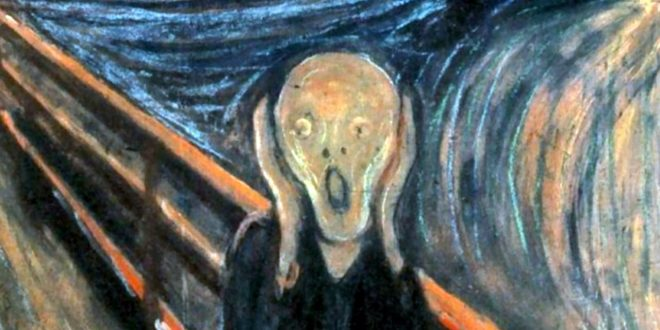
\includegraphics[width=\paperwidth]{munch2.jpg}
%}
%\begin{frame}
%\end{frame}
%}

%\section{Введение в Haskell}


%\defverbatim[colored]{\imageA}{
%\begin{tikzpicture}
%    [%%%%%%%%%%%%%%%%%%%%%%%%%%%%%%
%        box/.style={rectangle,draw=black, ultra thick, minimum size=1cm},
%    ]%%%%%%%%%%%%%%%%%%%%%%%%%%%%%%
%
%\foreach \x/\y in {0/9, 1/\faAmazon,2/13,3/19,4/12,5/8,6/7,7/4,8/21,9/2,10/6,11/11}
%        \node[box] at (\x,0){\y};
%
%\end{tikzpicture}
%}


\begin{frame}{Введение: $\lambda$-исчисление}
  \begin{figure}
    \centering
    \begin{subfigure}[t]{0.45\textwidth}
      \begin{minipage}{0.7\textwidth}
      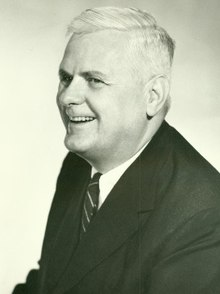
\includegraphics[width=1\textwidth]{220px-Alonzo_Church.jpg}\\
            Alonzo Church (1903–1995)
      \end{minipage}
    \end{subfigure}
    \begin{subfigure}[t]{0.45\textwidth}
      \vspace{-5em}   % TODO: dirty hack!
  Алонзо Чёрч 1935   открыл $\lambda$-исчисление
\vspace{1em}

Аналогичный подход от А.~Тьюринга с его машинами Тьюринга
\vspace{1em}

Это разные подходы для формализации понятия ``алгоритм''
\vspace{1em}

В принципе, могло быть изобретено уже в 1910-х г.г.
\footnotetext{Изображение из \href{https://en.wikipedia.org/wiki/Alonzo\_Church}{Википедии}}

    \end{subfigure}
  \end{figure}

%\thisfloatsetup{heightadjust=all,valign=t}
%\begin{figure}
%  \begin{subfloatrow}
%    \ffigbox[\dimexpr\FBwidth+4cm\relax]
%    {\includegraphics[width=3cm,height=5cm]{example-image-b}}
%    {\caption{Left subfigure}\label{sfig:testa}}%
%    \ffigbox[\FBwidth]
%    {\caption{Right subfigure}\label{sfig:testb}}
%    {\includegraphics[width=3cm,height=2cm]{example-image-a}}
%  \end{subfloatrow}
%\end{figure}

\end{frame}

\begin{frame}{Состояние математики в 1910-х}

    Матан, алгебра, геометрия...\\
    Информатики (computer science) явным образом пока нет, как часть математики\\

    Математическая логика
    \begin{enumerate}
      \item Пытается формализовать интуитивно понятные утверждения
      \item Языки (т.е. синтаксис), чтобы на них можно было правильно сформулировать теоремы
      \item Различные ``семантики'' как интерпретации синтаксиса , потому что формулы могут быть верны и не верны в зависимости от семантики
      \item ``Исчисления'' -- правильные способы доказательств
      \item Теоремы, которые невозможно ни доказать, ни опровергнуть.
    \end{enumerate}
  Начинают задумываться, что такое ``алгоритм'', ``вычисление'' и ``вычислимая функция''

\end{frame}

\begin{frame}{Зачем формализовывать то, что и так понятно?}
\framesubtitle{''Наивная'' теория множеств}
\begin{figure}[t]
  \begin{subfigure}[t]{0.55\textwidth}
    \vspace{-7em}
  Множества можно делить на два типа
  \begin{enumerate}
    \item   набор не является элементом самого себя
    \item Расселовские: набор является элементом самого себя.
  \end{enumerate}
  Рассмотрим $P=\{y: y\notin P\}$ и задумаемся про $P\in P$?
  \begin{itemize}
    \item Если формула верна, то нарушается определение
    \item Если ложна, то не принадлежит, но по определению должна
  \end{itemize}
\footnotetext{Изображение из \href{https://en.wikipedia.org/wiki/Bertrand\_Russell}{Википедии}}

  \end{subfigure}
\hspace{0.05\textwidth}
  \begin{subfigure}[t]{0.35\textwidth}
      \begin{minipage}{0.7\textwidth}
  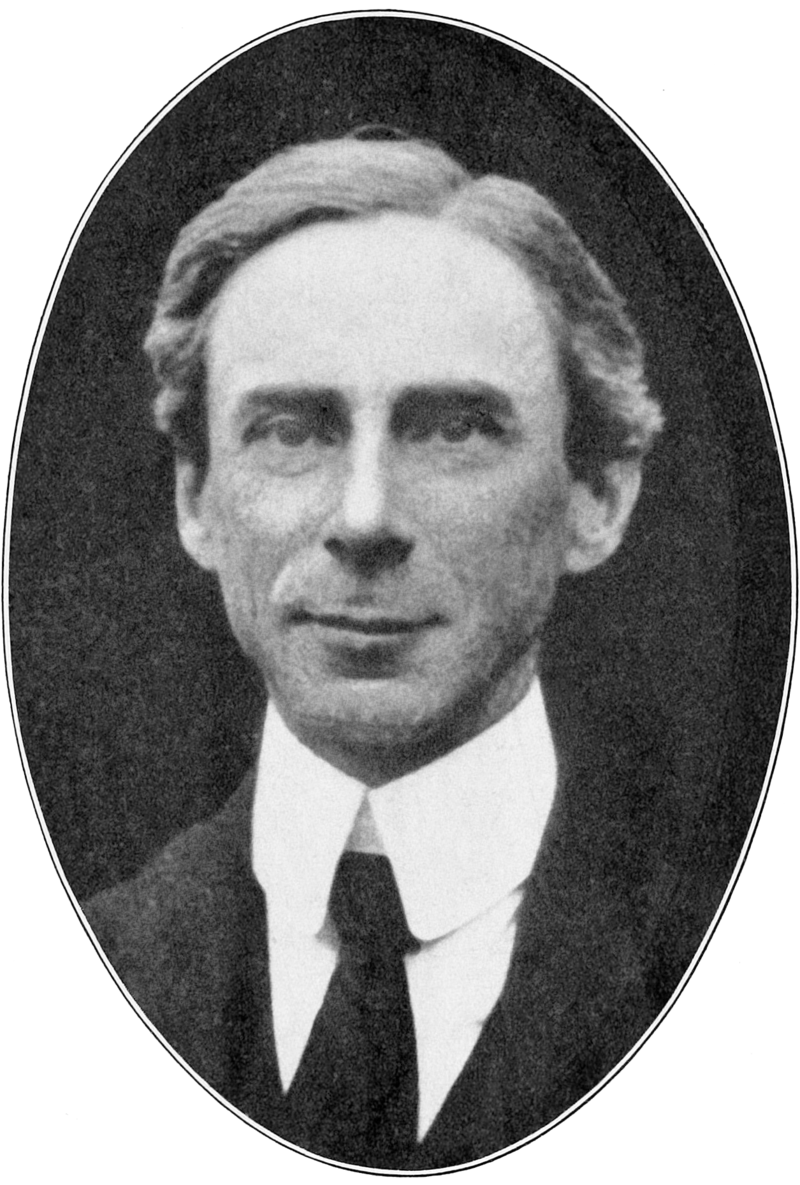
\includegraphics[width=1\textwidth]{800px-Bertrand_Russell_transparent_bg.png}\\
  Bertrand Russell (1872–1970)
\end{minipage}
  \end{subfigure}
\end{figure}
\end{frame}

\begin{frame}{Некоторые известные языки и исчисления из математической логики}
\begin{itemize}
  \item Нулевого порядка (высказываний)
  \item Первого порядка (предикатов)
  \item Высших порядков
  \item Исчисление конструкций (calculus of constructions)
\end{itemize}
\begin{block}{Важное замечание}
  То, что нельзя записать в языке, нельзя использовать в исчислениях/доказательствах
\end{block}
\end{frame}

\begin{frame}{Пример: яызк 0го порядка (высказываний) }
\frametitle{Знакомая вам булева (бинарная) логика}
\begin{figure}[t]
  \begin{subfigure}[t]{0.45\textwidth}
\begin{enumerate}
  \item Логические константы True и False
  \item Логические переменные $x,y,z,\dots$
  \item Бинарные связки $\vee, \wedge, \Rightarrow$ и т.д.
\end{enumerate}
\vspace{2em}
Правила вывода в исчислении, например:
\begin{mathpar}
  \inferrule* [Right=modus ponens]
  { P\Rightarrow Q \\    P  }{Q}
\end{mathpar}
  \end{subfigure}
\hspace{0.05\textwidth}
  \begin{subfigure}[t]{0.46\textwidth}
\begin{theorem}[Язык и исчисление \textbf{``хорошие''}]
  Верную формулу можно доказать за конечное число шагов. Ложную можно опровергнуть.\\

  Т.е. существует алгоритм, который всегда завершается и говорит да/нет.
\end{theorem}
\vspace{2em}
Язык и исчисление \textbf{``плохие''}, потому что не всё можно записать (где кванторы?)
  \end{subfigure}
\end{figure}


\end{frame}


\begin{frame}{Разрешимые и неразрешимые задачи}
  \begin{definition}[Алгоритмически неразрешимая задача]
    Задача, которая имеет ответ ``да'' или ``нет'', но для которое невозможно реализовать алгоритм, который \emph{всегда завершается, и выдает правильный ответ}.
  \end{definition}
  \begin{definition}[Полуразрешимая задача]
    Неразрешимая задача, для которой можно предъявить алгоритм, который либо дает правильный ответ  ``да'', либо не завершается. Полуразрешимые$^{+}$ умеют говорить ``да'', полуразрешимые$^{-}$ --- ``нет''.
  \end{definition}
Как доказывать неразрешимость
\begin{itemize}
  \item Разбирать случаи и искать противоречие в каждом
  \item Сводить каноничную неразрешимую задачу к нашей
\end{itemize}
\end{frame}

\begin{frame}{Язык и исчисление 1-го порядка (предикатов)}
%\framesubtitle{Вы это видели на матане}
\begin{figure}[t]
  \begin{subfigure}[t]{0.5\textwidth}
    Термы:
    \begin{itemize}
      \item Предметные константы: 1.0, 42, $\pi$
      \item Функциональные символы арности  $1\leqslant n$ от термов. Например, $+, \times, f, mod$ и т.д.
    \end{itemize}
    Формулы:
    \begin{itemize}
  \item Логические константы True и False
  \item Логические переменные $x,y,z,\dots$
  \item Бинарные связки $\vee, \wedge, \Rightarrow$ (и т.д.) %(от двух формул)
  \item Предикатные символы (от термов) арности $1\leqslant n$
  \item Кванторы $\forall, \exists$ от имени предметной переменной и формулы
    \end{itemize}
  \end{subfigure}
\hspace{0.05\textwidth}
  \begin{subfigure}[t]{0.4\textwidth}
    \begin{block}{Важно}
      $+, \times, f, mod$ это названия функциональных символов, никто не гарантирует, что  $+$ это сложение чисел
    \end{block}
\vspace{1em}
Пример: \\
$\forall x z\ \exists y (x < y) \vee (y < z)$\\
верно, если $x,y,z \in \mathbb{R}$, \\
неверно, если $x,y,z \in \mathbb{N}$
  \end{subfigure}
\end{figure}
\end{frame}

\begin{frame}{Преимущества и недостатки языка 1го порядка}

  \begin{itemize}
    \item Для некоторых формул из синтаксиса можно понять, что они верны (общезначимы). Для них есть алгоритм, который их докажет за конечное число шагов (см. ``метод британского музея'')
    \item Огромное количество формул верны только в некоторой семантике, для них нельзя предъявить, алгоритм, который завершается и выдает вердикт.\\
    В общем виде проверка формулы на истинность/ложность -- неразрешимая задача
    \item Язык недостаточно богат. Кванторы пробегают только предметные переменные, нельзя выразить ``для любой формулы P, верно...'', например, принцип индукции
    \[
    \forall P.\quad P(0) \Rightarrow (\forall n . P(n) \Rightarrow P(n+1))  \Rightarrow (\forall n . P(n))
    \]
  \end{itemize}
\end{frame}


%\begin{frame}{Недостатки исчисления предикатов}
%Некоторые формулы нельзя записать, а следовательно, пользоваться ими при доказательстве
%
%Например, принцип индукции
%
%
%
%Для этого нужен язык более высокого порядка, чем первого, а там всё ещё хуже с разрешимостью/неразрешимостью
%\end{frame}

\section{Лямбды как апгрейд языка предикатов}

\begin{frame}{Но можно попробовать вывернуться}
\framesubtitle{Введем специальный синтаксис}

\[
\lambda P.\quad phormula(P)
\]
Опишем принцип индукции, и применим его для $P(n)\equiv 0+\dots+n=\frac{n\cdot(n+1)}{2}$
\[
\lambda P.\quad P(0) \Rightarrow \big{(}\forall n . P(n) \Rightarrow P(n+1)\big{)}  \Rightarrow \big{(}\forall n . P(n)\big{)}
\]\pause
\[
\text{применение/подстановка} \mathlarger{\mathlarger{\mathlarger{\mathlarger{\Downarrow  \quad\!\!\!\!\!\!\Uparrow}}}} \text{абстракция}
\]

\begin{equation} \label{eq1}
  \begin{split}
    (0\equiv0) & \Rightarrow (\forall n . (0+\dots+n=\frac{n\cdot(n+1)}{2}) \Rightarrow \Big{(}0+\dots+(n+1)=\frac{(n+1)\cdot(n+2)}{2}\Big{)})  \\
    & \Rightarrow (\forall n . 0+\dots+n=\frac{n\cdot(n+1)}{2})
  \end{split}
\end{equation}
\end{frame}



\begin{frame}{Правила работы с новым языком $\lambda$}
\begin{block}{$\alpha$-эквивалентность}
При выборе новых имен, они не должны случайно перекрыть старые.\\
Предложения языка, отличающиеся только переименованием переменных, считаются ($\alpha$)эквивалентными
\end{block}
Например:  если ни $P$, ни $Q$ не встречаются в $phormula$, то $\lambda P. phormula(P)  \alphaequiv{} \lambda Q. phormula(Q) $

\begin{block}{$\beta$-эквивалентность}
Если у нас встречается $(\lambda P. phormula(P))X$, то мы можем продолжить с этим работать совершив подстановку $X$ вместо $P$ в $phormula$ (записывается как $phormula[P\mapsto X]$), т.е. заменив все свободные вхождения $P$ на $X$ внутри $phormula$.
\end{block}
\end{frame}


\begin{frame}{$\lambda$-исчисление}
Синтаксис
\begin{itemize}
  \item переменные: $x,y,z,\dots$
  \item Абстракция $(\lambda \nu. A)$, где $A$ -- $\lambda$-выражение, а $\nu$ --- произвольное имя переменной
  \item Применение $(AB)$, где $A$ и $B$ --- $\lambda$-выражения
\end{itemize}
\begin{definition}{Редекс}
  --- это $\lambda$-выражение вида $(\lambda \nu. A)B$
\end{definition}
Процесс вычисления --- это процеcc устранения редексов (возможно, не всех) путём подстановок $\lambda$-выражений вместо переменных.
\end{frame}

\begin{frame}{Каррирование%\footnote{}
  }

\begin{figure}[t]
  \begin{subfigure}[t]{0.5\textwidth}
    \vspace{-4em}
В $\lambda$-исчислении функция $n$ аргументов представляются как функция одного аргумента, которые возвращает функцию от $n-1$ аргумента.\\

В мире названо в честь Хаскеля Карри. Впервые появилось в 1924 в работе М.~И.~Шейнфинкеля.\\

\footnotetext{Изображение взято с \href{https://en.wikipedia.org/wiki/Moses\_Sch\%C3\%B6nfinkel}{Википедии}}

  \end{subfigure}
\hspace{1cm}
  \begin{subfigure}[t]{0.3\textwidth}
      \begin{minipage}{1\textwidth}
  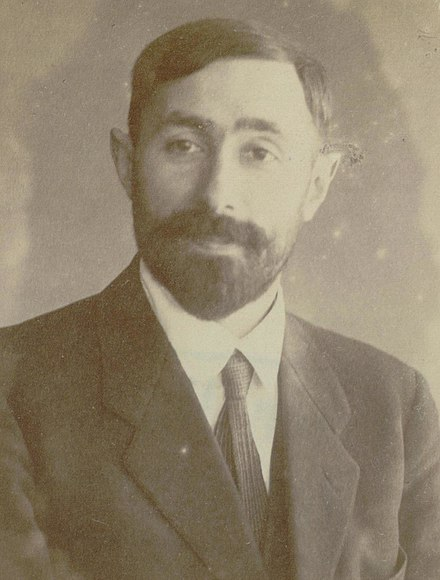
\includegraphics[width=1\textwidth]{440px-Moses_Schonfinkel_1922_(cropped).jpg}\\
  Моисей Исаевич Шейнфинкель (1888 -- 1942)
\end{minipage}
  \end{subfigure}
\end{figure}
\end{frame}


\begin{frame}{Определения алгоритма}
 \begin{theorem}[Тезис Чёрча]
  Используя $\lambda$-исчисление можно реализовать произвольный алгоритм
  \emph{с точностью до представления данных}.
\end{theorem}
\begin{theorem}[Тезис Тьюринга]
Используя машину Тьюринга можно реализовать произвольный алгоритм
\emph{с точностью до представления данных}.
\end{theorem}
Т.е. теперь под алгоритмом понимается только то, что можно записать в формализме.
\end{frame}

\begin{frame}{Как происходят вычисления (редукция) $\lambda$-исчислении?}
  \begin{definition}[Процесс вычислений регламентирует стратегия]
    Ищем редексы $(\lambda x. P)Q$
    \begin{itemize}
      \item Если редексов нет, то вычисление закончилось
      \item Если редексы есть, стратегия регламентирует какой на данном шаге редекс стоит $\beta$-редуцировать
      \item Или же, стратегия может сказать, что все редексы нужно оставить как есть, и выдать ответ.
    \end{itemize}
  \end{definition}
  %Стратегий бывает много разных
  %\begin{enumerate}
  %  \item Строгая стратегия call-by-value .    Для $(\lambda x. P)Q$ вычисляет $Q\cbv Q'$ и потом подставляет $Q'$ вместо $x$ в $P$.
  %  \item Ленивая стратегия call-by-name.   Для $(\lambda x. P)Q$ сразу подставляет $Q$ вместо $x$ в $P$.
  %  \item Обе стратегии оставляют абстракции и переменные как есть
  %\end{enumerate}
\end{frame}

\begin{frame}{Две стратегии: Call-by-value и аппликативная}
  \begin{figure}[t]
    \begin{subfigure}[t]{0.45\textwidth}
            \centering Call-by-value
      \begin{mathpar}
  \inferrule*  [Right=Abs] {\\}
{\lam{x}{e} \cbv \lam{x}{e}}
\end{mathpar}
    \end{subfigure}
    \begin{subfigure}[t]{0.45\textwidth}
      \centering
      Applicative order
      \begin{mathpar}
      \inferrule* [Right=Abs] {e \ao e'}
      {\lam{x}{e} \ao \lam{x}{e'}}
      \end{mathpar}
    \end{subfigure}
  \end{figure}
\hrulefill
\only<1>{
\begin{mathpar}
  \inferrule*  [Right=App-abs]
  { e_1 \arr \lam{x}{e} \\
    e_2 \arr e_2' \\
    [e_2'/x]e \arr e'
  }
  { (e_1 e_2) \arr e'}
\end{mathpar}
\begin{mathpar}
  \inferrule* [Right=Var] {\\}
  {x \arr x}
  \and
  \inferrule*  [Right=App-non-abs]
  { e_1 \arr e' \neq \lam{x}{e} \\
    e_2 \arr e_2'}
  { (e_1 e_2) \arr (e_1' e_2') }
\end{mathpar}
}
\only<2>{
\begin{figure}[t]
  \begin{subfigure}[t]{0.45\textwidth}
\begin{itemize}
\item[\faGood]    Подходит для написания произвольных алгоритмов
\vspace{4em}

\item[\faBad] Не считает под абстракцией, поэтому ответ иногда длиннее, чем хотелось бы
\end{itemize}
  \end{subfigure}
  \begin{subfigure}[t]{0.45\textwidth}
\begin{itemize}
  \item[\faBad] Нет возможности отложить вычисления на потом,т.е. в if-then-else вычисляется и then, и else. Нельзя дождаться ответа от рекурсивных функций
  \item[\faGood] Cчитает под абстракцией, поэтому ответ короче
\end{itemize}
  \end{subfigure}
\end{figure}
}
\end{frame}


\section{Написание алгоритмов с помощью $\lambda$-исчисления}

\begin{frame}{Что нужно для представления алгоритмов?}
  \begin{itemize}
    \item Принимать входные данные
    \item Делать ветвления  в зависимости от входных данных
    \item Совершать некоторое количество однотипных действий в зависимости от входных данных (т.е. должны быть циклы или их аналог -- рекурсия)
    \begin{itemize}
\item       Чтобы понимать, сколько действий уже сделали нужны натуральные числа
    \end{itemize}
  \end{itemize}
\end{frame}

\begin{frame}{Ветвления}
\[
T\equiv\lam{x}{\lam{y}{x}} \equiv fst \qquad \qquad \qquad \qquad
F\equiv \lam{x}{\lam{y}{y}}\equiv snd
\]

\begin{align*}
  ite \quad\equiv &\quad \lambda c. \lambda th. \lambda el. (c\ th\ el)\\
  (ite\ T) \quad\equiv &\quad  \lambda th. \lambda el. (T\ th\ el) \rightsquigarrow th\\
  (ite\ F) \quad\equiv &\quad  \lambda th. \lambda el. (F\ th\ el) \rightsquigarrow el
\end{align*}
\end{frame}

%\section{Представление данных в $\lambda$ исчислении}
\begin{frame}{Представление чисел (Нумералы Чёрча)}

  $ 0 \sim \lam{s}{\lam{x}{x}}$

  $ 1 \sim \lam{s}{\lam{x}{sx}}$

  $ 2 \sim \lam{s}{\lam{x}{s(sx)}}$

  и т.д.
  \vspace{1cm}

  Сложение (один из вариантов): взять два нумерала $m$ и $n$, взять $f$ и $x$, а затем к $x$ применить $n$ раз $f$, а затем к результату применить $m$ раз $f$.

  \[
  add \equiv \lambda m. \lambda n. \lambda f. \lambda x. \app{m\ f\ }{\app{n\ f\ }{x}}
  \]
\end{frame}
\newcommand{\tb}[1]{\textcolor{blue}{#1}}
\newcommand{\tr}[1]{\textcolor{red}{#1}}
\begin{frame}{2+2}
  \begin{align*}
    (\lambda m. \lambda n. \lambda f. \lambda x. \app{m\ f\ }{\app{n\ f\ }{x}}){} 2 2 &\cbv \\
    \textcolor{blue}{(\lambda m. \lambda n. \lambda f. \lambda x. \app{m\ f\ }{\app{n\ f\ }{x}}) {}} \textcolor{red}{2} 2 &\cbv \\
    \textcolor{blue}{( \lambda n. \lambda f. \lambda x. \app{2\ f\ }{\app{n\ f\ }{x}}){}} \textcolor{red}{2} & \cbv \\
    \lambda f. \lambda x. \app{2\ f\ }{\app{2\ f\ }{x}}   &\xarr{\ \ } \\
    \lambda f. \lambda x. \app{\tb{\lam{f}{\lam{x}{f (f x)}}} \ \tr{f}\ }{\app{2\ f\ }{x}} &\ao \\
    \lambda f. \lambda x. \app{\lam{x}{f (f x)} \ \ }{\app{2\ f\ }{x}} &\xarr{\ \ } \\
    \lambda f. \lambda x. \app{\lam{x}{f (f x)} \ \ } {\app{\app{\tb{\lam{f}{\lam{x}{f (f x)}}}\ \tr{f}\ }{x}}} &\ao \\
    \lambda f. \lambda x. \app{\lam{x}{f (f x)}  } {\app{\tb{\lam{x}{f (f x)} } }{\tr{x}}} &\ao \\
    \lambda f. \lambda x. \app{\tb{\lam{x}{f (f x)} } } {\tr{(f (f x))}} &\ao \\
    \lambda f. \lambda x. \lam{x}{f (f (f (f x)))} &
  \end{align*}
\end{frame}


\begin{frame}{2+2}
  \begin{figure}[t]
    \begin{subfigure}[t]{0.50\textwidth}
      \begin{align*}
        (\lambda m. \lambda n. \lambda f. \lambda x. \app{m\ f\ }{\app{n\ f\ }{x}}){} 2 2 &\cbv \\
        \textcolor{blue}{(\lambda m. \lambda n. \lambda f. \lambda x. \app{m\ f\ }{\app{n\ f\ }{x}}) {}} \textcolor{red}{2} 2 &\cbv \\
        \textcolor{blue}{( \lambda n. \lambda f. \lambda x. \app{2\ f\ }{\app{n\ f\ }{x}}){}} \textcolor{red}{2} & \cbv \\
        \lambda f. \lambda x. \app{2\ f\ }{\app{2\ f\ }{x}}   &
      \end{align*}
      Это ответ для $\cbv$.\\

      Давайте посмотрим, что будет, если мы \\
      ответ применим к $g$ и $y$
    \end{subfigure}
    \begin{subfigure}[t]{0.45\textwidth}
      \begin{align*}
        (\lambda f. \lambda x. \app{2\ f\ }{\app{2\ f\ }{x}}) g y  &\cbv \\
        (\lambda x. \app{2\ g\ }{\app{2\ g\ }{x}}) y  &\cbv \\
        \app{2\ g\ }{\app{2\ g\ }{y}}   &\cbv \\
        \app{\tb{\lam{f}{\lam{x}{f (f x)}}} \ \tr{g}\ }{\app{2\ g\ }{y}} &\cbv \\
        \app{\lam{x}{g (g x)} \ \ }{\app{2\ g\ }{y}} &\cbv \\
        \app{\lam{x}{g (g x)} \ \ } {\app{\app{\tb{\lam{f}{\lam{x}{f (f x)}}}\ \tr{g}\ }{x}}} &\cbv \\
        \app{\lam{x}{g (g x)}  } {\app{\tb{\lam{x}{g (g x)} } }{\tr{y}}} &\cbv \\
        \app{\tb{\lam{x}{g (g x)} } } {\tr{(g (g y))}} &\cbv \\
        g (g (g (g y))) &
      \end{align*}
    \end{subfigure}
  \end{figure}
\end{frame}

\begin{frame}{Рекурсия}
Не понятно как вызвать самого себя, так как имен нет.\\

Идея:
\begin{itemize}
  \item записываем фунцию $f$, чтобы она принимала первый аргумент, который будет вызываться вместо рекурсивного вызова
  \item Везде, где надо вызвать эту ``рекурсивную'' функцию, будем писать $Yf$  или $Zf$

  $$
  Y\equiv \lam{f}{\lam{x}{f(x\ x)}\lam{x}{f(x\ x)}}
  $$

  $$
  Z\equiv \lam{f}{\lam{x}{f\lam{v}{\ x\ x\ v}}\lam{x}{f\lam{v}{\ x\ x\ v}}}
  $$
\end{itemize}

\end{frame}


\newcommand{\ite}[3]{\ensuremath{(\text{if } #1\text{ then }#2\text{ else }#3})}}
\begin{frame}{Рекурсия в call-by-value (упрощенно)}
$$
Z\equiv \lam{f}{\lam{x}{f\lam{v}{\ x\ x\ v}}\lam{x}{f\lam{v}{\ x\ x\ v}}}
$$
%Основное свойство
\[
ZR = \lam{x}{R\lam{v}{\ x\ x\ v}} \lam{x}{R\lam{v}{\ x\ x\ v}} \nor
R\big( \lam{x}{R\lam{v}{\ x\ x\ v}}\lam{x}{R\lam{v}{\ x\ x\ v}} \big) =
R(ZR)
\]

\vspace{1em}

Факториал: $fac \equiv (\lambda self.\lambda n . \ite{n<2}{1}{n \cdot self(n-1)})$
\begin{align*}
  Z(\lambda self.\lambda n . \ite{n<2}{1}{n \cdot self(n-1)}) 2 &\cbn \\
  (\lambda n . \ite{n<2}{1}{n \cdot Z\ fac(n-1)}) 2 &\cbn \\
  2 \cdot Y\ fac\ (2-1) &\cbn \\
  2 \cdot (Z(\lambda self.\lambda n . \ite{n<2}{1}{n \cdot self(n-1)})\ 1) &\cbn \\
  2 \cdot \ite{1<2}{1}{n \cdot (Z\ fac\ (1-1))} &\cbn \\
  2 \cdot 1 & \cbn 2
\end{align*}
\end{frame}

%\section{Две стратегии}
\begin{comment}

\begin{frame}{Как происходят вычисления (редукция) $\lambda$-исчислении?}
\begin{definition}[Процесс вычислений регламентирует стратегия]
  Ищем редексы $(\lambda x. P)Q$
\begin{itemize}
  \item Если редексов нет, то вычисление закончилось
  \item Если редексы есть, стратегия регламентирует какой на данном шаге редекс стоит $\beta$редуцировать
  \item Или же, стратегия может сказать, что все редексы нужно оставить как есть, и выдать ответ.
\end{itemize}
\end{definition}
%Стратегий бывает много разных
%\begin{enumerate}
%  \item Строгая стратегия call-by-value .    Для $(\lambda x. P)Q$ вычисляет $Q\cbv Q'$ и потом подставляет $Q'$ вместо $x$ в $P$.
%  \item Ленивая стратегия call-by-name.   Для $(\lambda x. P)Q$ сразу подставляет $Q$ вместо $x$ в $P$.
%  \item Обе стратегии оставляют абстракции и переменные как есть
%\end{enumerate}
\end{frame}

\begin{frame}{Ленивая vs. Строгая}
Пример 1 ($\cbv$ выглядит лучше)\\
$(\lambda x. f x x)((\lambda x. x)A) \cbv (\lambda x. f x x)A \cbv (f A A) \cbv \dots $\\

$(\lambda x. f x x)((\lambda x. x)A) \cbn (\lambda x. f ((\lambda x. x)A) ((\lambda x. x)A))A \cbn \dots $

\vspace{3em}
Пример 2 ($\cbn$ выглядит лучше)\\
$(\lambda x. \lambda y. y)((\lambda x. xx)(\lambda x. xx)) \cbv (\lambda x. \lambda y. y)((\lambda x. xx)(\lambda x. xx)) \cbv \dots \text{зависло}$

$(\lambda x. \lambda y. y)((\lambda x. xx)(\lambda x. xx)) \cbn (\lambda y. y)\quad\text{ответ!}$
\end{frame}
\end{comment}



\begin{comment}


\newcommand{\ite}[3]{\ensuremath{(\text{if } #1\text{ then }#2\text{ else }#3})}}
\begin{frame}{Рекурсия в call-by-name}
$$
Y\equiv \lam{f}{\lam{x}{f(xx)}\lam{x}{f(xx)}}
$$
%Основное свойство
\[
YR = \lam{x}{R(xx)} \lam{x}{R(xx)} \nor
R\big( \lam{x}{R(xx)}\lam{x}{R(xx)} \big) =
R(YR)
\]

\vspace{1em}

Факториал: $fac \equiv (\lambda self.\lambda n . \ite{n<2}{1}{n \cdot self(n-1)})$
\begin{align*}
  Y(\lambda self.\lambda n . \ite{n<2}{1}{n \cdot self(n-1)}) 2 &\cbn \\
  (\lambda n . \ite{n<2}{1}{n \cdot Y\ fac(n-1)}) 2 &\cbn \\
   2 \cdot Y\ fac\ (2-1) &\cbn \\
   2 \cdot (Y(\lambda self.\lambda n . \ite{n<2}{1}{n \cdot self(n-1)})\ 1) &\cbn \\
   2 \cdot \ite{1<2}{1}{n \cdot (Y\ fac\ (1-1))} &\cbn \\
  2 \cdot 1 & \cbn 2
\end{align*}

\end{frame}
\end{comment}


\section{Демка интерпретатора на Си}
\begin{frame}{Дэмка на Си}
  Не забыть показать позднее связывание
\end{frame}

\section*{Вопросы к экзамену (TODO)}
\begin{frame}{Вопросы к экзамену}
\begin{enumerate}
  \item Разрешимые и неразрешимые задачи
  \item $\lambda$-исчисление. $\alpha$ и $\beta$ правила
  \item Нумералы Чёрча. Сложение
  \item Рекурсия и факториал
\end{enumerate}
\end{frame}

%
%\begin{frame}%{Чистые функции}
%\begin{definition}[Неизменяемые структуры данных (immutable data structures)]
%  Которые с течением времени не изменяются \faSmileO
%\end{definition}
%
%\vspace{1em}
%
%\begin{definition}[Устойчивые структуры данных (persistent data structures)]
%Имеют доступ (не уничтожают) предыдущее своё состояние
%\end{definition}
%Почти то же самое, только акцент смещён\vspace{1em}
%
%\begin{remark}
%Так как старые узлы есть, то можно их использовать (share) в новой версии структуры данных
%\end{remark}
%\begin{definition}[Неустойчивые структуры данных называются \textit{эфемерными (ephemeral)}]
%\end{definition}
%\end{frame}



\section{Списки}

%\section{Ленивое вычисление}


%\chap{Основы амортизации}


\section{Методы амортизированного анализа}
\label{sc:5.1}


\begin{frame}{Методы амортизированного анализа}
Реализации с амортизированными
характеристиками производительности часто оказываются проще и быстрее,
чем реализации со сравнимыми жёсткими характеристиками. \\

К сожалению, простой подход к амортизации, рассматриваемый в этой
главе, конфликтует с идеей устойчивости~--- эти структуры, будучи
используемы как устойчивые, могут быть весьма неэффективны. Однако на
практике многие приложения устойчивости не требуют, и часто для таких
приложений реализации, представленные в этой главе, могут быть
замечательным выбором. \\

Чтобы совместить амортизацию и устойчивость стоит применить 
\emph{ленивые вычисления}.

%В следующей главе мы увидим, как можно
%совместить понятия амортизации и устойчивости при помощи ленивого
%вычисления.
%
%TODO:
\end{frame}


\begin{frame}[fragile]{}
Понятие амортизации возникает из следующего наблюдения.  Имея
последовательность операций, мы можем интересоваться временем, которое
отнимает вся эта последовательность, однако при этом нам может быть
безразлично время каждой отдельной операции.\\

 Например, имея $n$
операций, мы можем желать, чтобы время всей последовательности было
ограничено показателем $O(n)$, не настаивая, чтобы каждая из этих
операций происходила за время $O(1)$. Нас может устраивать, чтобы
некоторые из операций занимали $O(\log n)$ или даже $O(n)$, при
условии, что общая стоимость всей последовательности будет
$O(n)$. \\

Такая дополнительная степень свободы открывает широкое
пространство возможностей при проектировании, и часто позволяет найти
более простые и быстрые решения, чем варианты с аналогичными жёсткими
ограничениями.

\end{frame}


\begin{frame}[fragile]{}
$$
\sum_{i=1}^m a_i \ge \sum_{i=1}^m t_i
$$
где $a_i$~--- амортизированная стоимость $i$-й операции, $t_i$~--- ее
реальная стоимость, а $m$~--- общее число операций.\\

 Обычно
доказывается несколько более сильный результат: что на любой
промежуточной стадии в последовательности операций общая текущая
амортизированная стоимость является верхней границей для общей текущей
реальной стоимости, т.~е. для любого $j$
$$
\sum_{i=1}^j a_i \ge \sum_{i=1}^j t_i
$$
\end{frame}


\begin{frame}[fragile]{}
\begin{definition}
Разница между общей текущей амортизированной стоимостью
и общей текущей реальной стоимостью называется
\term{текущие накопления}{accumulated savings}. 
\end{definition}
Таким образом, общая
текущая амортизированная стоимость является верхней границей для
общей текущей реальной стоимости тогда и только тогда, когда текущие
накопления неотрицательны.

\end{frame}


\begin{frame}[fragile]{}
Амортизация позволяет некоторым операциям быть дороже, чем их
амортизированная стоимость. Такие операции называются
\term{дорогими}{expensive}. Операции, для которых амортизированная
стоимость превышает реальную, называются
\term{дешевыми}{cheap}. Дорогие операции уменьшают текущие накопления,
а дешевые их увеличивают.\\

 Главное при доказательстве
амортизированных характеристик стоимости~--- показать, что дорогие
операции случаются только тогда, когда текущих накоплений хватает,
чтобы покрыть их дополнительную стоимость.
\end{frame}



\begin{frame}[fragile]{}
\begin{itemize}
  \item \term{Метод банкира}{banker's method} 
      \begin{itemize}
        \item \term{кредит}{credits}
      \end{itemize}
  \item \term{Метод физика}{physicist's method}
      \begin{itemize}
        \item \term{потенциал}{potential}
      \end{itemize}
\end{itemize}



Кредит и потенциал являются лишь средствами анализа; ни
то, ни другое не присутствует в тексте программы (разве что, возможно,
в комментариях).

\end{frame}

\begin{frame}[fragile]{}
 В методе банкира
текущие накопления представляются как \term{кредит}{credits},
привязанный к определенным ячейкам структуры данных. Этот кредит
используется, чтобы расплатиться за будущие операции доступа к этим
ячейкам.  Амортизированная стоимость операции определяется как ее
реальная стоимость плюс размер кредита, выделяемого этой операцией,
минус размер кредита, который она расходует, т.~е.,
$$
a_i = t_i + c_i - \bar{c}_i
$$
где $c_i$~--- размер кредита, выделяемого операцией $i$, а $\bar{c}_i$~---
размер кредита, расходуемого операцией $i$.


\end{frame}

\begin{frame}[fragile]{}
$$
a_i = t_i + c_i - \bar{c}_i
$$
где $c_i$~--- размер кредита, выделяемого операцией $i$, а $\bar{c}_i$~---
размер кредита, расходуемого операцией $i$.\\

 Каждая единица кредита
должна быть выделена, прежде чем израсходована, и нельзя расходовать
кредит дважды. Таким образом, $\sum c_i \ge \sum \bar{c}_i$, а
следовательно, как и требуется, $\sum a_i \ge \sum t_i$.\\

Как правило,
доказательства с использованием метода банкира определяют
\term{инвариант кредита}{credit invariant}, регулирующий распределение
кредита так, чтобы при всякой дорогой операции достаточное его
количество было выделено в нужных ячейках структуры для покрытия
стоимости операции.
\end{frame}

\begin{frame}[fragile]{Метод физика}
Определяется функция $\Phi$, отображающая всякий
объект $d$ на действительное число, называемое его
\term{потенциалом}{potential}.  Потенциал обычно выбирается так, чтобы
изначально равняться нулю и оставаться неотрицательным. В таком случае
потенциал представляет нижнюю границу  текущих накоплений.\\

Пусть объект $d_i$ будет результатом операции $i$ и аргументом
операции $i+1$. Тогда амортизированная стоимость операции $i$
определяется как сумма реальной стоимости и изменения потенциалов между
$d_{i-1}$ и $d_i$, т.~е.,
$$
a_i = t_i + \Phi(d_i) - \Phi(d_{i-1})
$$
текущих накоплений.


\end{frame}


\begin{frame}[fragile]{}
$$
a_i = t_i + \Phi(d_i) - \Phi(d_{i-1})
$$
Текущая реальная стоимость последовательности операций равна
$$
\begin{array}{rcl}
\sum_{i=1}^j t_i & = & \sum_{i=0}^j (a_i + \Phi(d_{i-1}) - \Phi(d_i))\\
\\
& = & \sum_{i=1}^j a_i + \sum_{i=1}^j (\Phi(d_{i-1}) - \Phi(d_i)) \\
\\
& = & \sum_{i=1}^j a_i + \Phi(d_0) - \Phi(d_j)
\end{array}
$$

Если $\Phi$ выбран таким образом, что
$\Phi(d_0)$ равен нулю, а $\Phi(d_j)$ неотрицателен, мы имеем
$\Phi(d_j) \ge \Phi(d_0)$, так что, как и требуется, текущая общая
амортизированная стоимость является верхней границей для текущей общей
реальной стоимости.

\end{frame}

\begin{comment}
\begin{remark}
Такое описание метода физика несколько упрощает
картину. Часто при анализе оказывается трудно втиснуть реальное
положение дел в указанные рамки. Например, что делать с функциями,
которые порождают или возвращают более одного объекта? Однако даже
упрощенное описание достаточно для демонстрации основных идей.
\end{remark}

\end{comment}

\section{Очереди}
\label{sc:5.2}


\begin{frame}[fragile]{}

\begin{minipage}{.4\textwidth}
  \inputminted[firstline=5,lastline=11] {haskell}{code/Queue.lhs}
\end{minipage}
\begin{minipage}{.55\textwidth}
  Самая распространенная чисто функциональная реализация очередей
  представляет собой пару списков, \hsinline{f} и \hsinline{r}, где
  \hsinline{f} содержит головные элементы очереди в правильном порядке,
  а \hsinline{r} состоит из хвостовых элементов в обратном порядке.\\
  
  Например, очередь, содержащая целые числа 1\ldots 6, может быть
  представлена списками \hsinline{f=[1,2,3]} и
  \hsinline{r=[6,5,4]}. Это представление можно описать следующим
  типом:
  \begin{minted}{haskell}
  data Queue a = Queue [a] [a]
  \end{minted}
  
\end{minipage}
\end{frame}


\begin{frame}[fragile]{}
В этом представлении голова очереди~--- первый элемент \hsinline{f},
так что функции \hsinline{head} и \hsinline{tail}
возвращают и отбрасывают этот элемент, соответственно.
\begin{minted}{haskell}
head (x : f, r) = x
tail (x : f, r) = f
\end{minted}
Подобным образом, хвостом очереди является первый элемент
\hsinline{r}, так что \hsinline{snoc} добавляет к \hsinline{r}
новый.
\begin{minted}{haskell}
snoc (f,r) x = (f, x : r)
\end{minted}

\end{frame}


\begin{frame}[fragile]{}
Элементы добавляются к \hsinline{r} и убираются из \hsinline{f}, так
что они должны как-то переезжать из одного списка в другой. Этот
переезд осуществляется путем обращения \hsinline{r} и установки его
на место \hsinline{f} всякий раз, когда в противном случае
\hsinline{f} оказался бы пустым.\\

 Одновременно \hsinline{r}
устанавливается в \hsinline{[]}. Наша цель~--- поддерживать
инвариант, что список \hsinline{f} может быть пустым только в том
случае, когда список \hsinline{r} также пуст (т.~е., пуста вся
очередь). \\

Заметим, что если бы \hsinline{f} был пустым при непустом
\hsinline{r}, то первый элемент очереди находился бы в конце
\hsinline{r}, и доступ к нему занимал бы $O(n)$ времени. Поддерживая
инвариант, мы гарантируем, что функция \hsinline{head} всегда может
найти голову очереди за $O(1)$ времени.

\end{frame}


\begin{frame}[fragile]{}
\begin{minted}{haskell}
snoc (([], _), x) = ([x], [])
snoc (( f, r), x) = (f,  x :: r)
tail ([x], r) = (rev r, [])
tail (x:f, r) = (f, r)
\end{minted}

Заметим, что в первой ветке \hsinline{snoc} используется
wildcard. В этом случае поле \hsinline{r} проверять не нужно,
поскольку из инварианта мы знаем, что если список \hsinline{f} равен
\hsinline{[]}, то \hsinline{r} также пуст.

\end{frame}


\begin{frame}[fragile]{}
Чуть более изящный способ записать эти функции~--- вынести те части
\hsinline{snoc} и \hsinline{tail}, которые поддерживают инвариант, в
отдельную функцию \hsinline{checkf}. Она заменяет \hsinline{f} на
\hsinline{rev r}, если \hsinline{f} пуст, а в противном случае
ничего не делает.

\inputminted[firstline=10,lastline=15] {haskell}{code/NaiveQueue.hs}

Функции
\hsinline{snoc} и \hsinline{head} всегда завершаются за время
$O(1)$, но \hsinline{tail} в худшем случае отнимает $O(n)$
времени. 

Однако, используя либо метод банкира, либо метод физика, мы
можем показать, что как \hsinline{snoc}, так и \hsinline{tail}
занимают амортизированное время $O(1)$.

\end{frame}


\begin{frame}[fragile]{Чисто функциональная очередь и метод банкира}

Инвариант: каждый элемент в
хвостовом списке связан с одной единицей кредита. \\

Каждый вызов
\hsinline{snoc} для непустой очереди занимает один реальный шаг и
выделяет одну единицу кредита для элемента хвостового списка; таким
образом, общая амортизированная стоимость равна двум. \\

Вызов
\hsinline{tail}, не обращающий хвостовой список, занимает один шаг,
не выделяет и не тратит никакого кредита, и, таким образом, имеет
амортизированную стоимость 1. \\

Наконец, вызов \hsinline{tail},
обращающий хвостовой список, занимает $m+1$ реальный шаг, где $m$~---
длина хвостового списка, и тратит $m$ единиц кредита, содержащиеся в
этом списке, так что амортизированная стоимость получается $m + 1 - m
= 1$.

\end{frame}


\begin{frame}[fragile]{Чисто функциональная очередь и метод физика}
В методе физика мы определяем функцию потенциала $\Phi$ как длину
хвостового списка. \\

Тогда всякий \hsinline{snoc} к непустой очереди
занимает один реальный шаг и увеличивает потенциал на единицу, так что
амортизированная стоимость равна двум. \\

Вызов \hsinline{tail} без
обращения хвостовой очереди занимает один реальный шаг и не изменяет
потенциал, так что амортизированная стоимость равна одному.\\

 Наконец,
вызов \hsinline{tail} с обращением очереди занимает $m+1$ реальный
шаг, но при этом устанавливает хвостовой список равным \hsinline{[]},
уменьшая таким образом потенциал на $m$, так что амортизированная
стоимость равна $m + 1 - m = 1$.

\end{frame}


\begin{frame}[fragile]{}
\begin{hint}
  Эта реализация очередей идеальна в приложениях, где не требуется
  устойчивости и где приемлемы амортизированные показатели
  производительности.
\end{hint}

\end{frame}

\ifanswers
\begin{frame}[fragile]{}
\begin{exercise}\label{ex:5.1}
  \textbf{Хогерворд \cite{Hoogerwoord1992}.}  Идея этих очередей легко
  может быть расширена на абстракцию \term{двусторонней очереди}{double-ended
    queue}, или \term{дека}{deque}, где чтение и запись разрешены с
  обоих концов очереди (см. Рис.~\ref{fig:5.3}). Инвариант делается
  симметричным относительно \lstinline!f! и \lstinline!r!: если
  очередь содержит более одного элемента, оба списка должны быть
  непустыми. Когда один из списков становится пустым, мы делим другой
  пополам и одну из половин обращаем.
  
  \begin{enumerate}
    \item Реализуйте эту версию деков.
    \item Докажите, что каждая операция занимает $O(1)$ амортизированного
    времени, используя функцию потенциала $\Phi(f,r) = abs(|f| -
    |r|)$, где $abs$~--- функция модуля.
  \end{enumerate}
\end{exercise}
\end{frame}
\fi

\section{Биномиальные кучи}
\label{sc:5.3}


\begin{frame}[fragile]{}
В Разделе~\ref{sc:3.2} мы показали, что вставка в биномиальную кучу
проходит в худшем случае за время $O(\log n)$. Здесь мы доказываем,
что на самом деле амортизированное ограничение на время вставки
составляет $O(1)$.\\

Метод физика. Потенциал биномиальной кучи -- число деревьев в ней. 

Заметим, что это число равно количеству
единиц в двоичном представлении $n$, числа элементов в куче.  Вызов
\hsinline{insert} занимает $k+1$ шаг, где $k$~--- число обращений к
\hsinline{link}. Если изначально в куче было $t$ деревьев, то после
вставки окажется $t - k + 1$ деревьев. Таким образом, изменение
потенциала составляет $(t - k + 1) - t = 1 - k$, а амортизированная
стоимость вставки $(k + 1) + (1 - k) = 2$.\\

\begin{exercise}\label{ex:5.2}
  Повторите доказательство с использованием метода банкира.
\end{exercise}

\end{frame}


\begin{frame}[fragile]{}
Для полноты картины нам нужно показать, что амортизированная стоимость
операций \hsinline{merge} и \hsinline{deleteMin} по-прежнему
составляет $O(\log n)$. \hsinline{deleteMin} не доставляет здесь
никаких трудностей, но в случае \hsinline{merge} требуется небольшое
расширение метода физика. \\

До сих пор мы определяли амортизированную
стоимость операции как
$$
a = t + \Phi(d_{\mbox{\textit{вых}}}) - \Phi(d_{\mbox{\textit{вх}}})
$$
где $d_{\mbox{\textit{вх}}}$~--- структура на входе операции, а $d_{\mbox{\textit{вых}}}$~---
структура на выходе. Однако если операция принимает либо возвращает
более одного объекта, это определение требуется обобщить до
$$
a = t + \sum_{d \in \mbox{\textit{Вых}}} \Phi(d) - \sum_{d \in \mbox{\textit{Вх}}} \Phi(d)
$$
где $\mbox{\textit{Вх}}$~--- множество входов, а $\mbox{\textit{Вых}}$~--- множество выходов. В этом
правиле мы рассматриваем только входы и выходы анализируемого типа.
\end{frame}

\ifanswers
\begin{frame}[fragile]{}
\begin{exercise}\label{ex:5.3}
  Докажите, что амортизированная стоимость операций \hsinline{merge}
  и \hsinline{deleteMin} по-прежнему составляет $O(\log n)$.
\end{exercise}
\end{frame}
\fi


\section{Расширяющиеся кучи}
\label{sc:5.4}

\begin{frame}{\term{Расширяющиеся деревья}{splay trees}}
\term{Расширяющиеся деревья}{splay trees} \cite{SleatorTarjan1985}~--- возможно, самая известная
и успешно применяемая амортизированная структура данных.\\

 Расширяющиеся
деревья являются ближайшими родственниками двоичных сбалансированных
деревьев поиска, но они не хранят никакую информацию о балансе
явно. \\

Вместо этого каждая операция перестраивает дерево при помощи
некоторых простых преобразований, которые имеют тенденцию увеличивать
сбалансированность. Несмотря на то, что каждая конкретная операция
может занимать до $O(n)$ времени, амортизированная стоимость ее, как
мы покажем, не превышает $O(\log n)$.
\end{frame}


\begin{frame}[fragile]{Расширяющиеся vs. деревья поиска}
Важное различие между расширяющимися и сбалансированными
двоичными деревьями поиска вроде красно-чёрных деревьев из
Раздела~\ref{sc:3.3} состоит в том, что расширяющиеся деревья
перестраиваются даже во время запросов (таких, как \hsinline{member}),
а не только во время обновлений (таких, как \hsinline{insert}). \\

Это
свойство мешает использованию расширяющихся деревьев для реализации
абстракций вроде множеств или конечных отображений в чисто
функциональном окружении, поскольку приходилось бы возвращать в
запросе новое дерево наряду с ответом на запрос\footnote{%
  В принципе можно было бы хранить корень расширяющегося дерева в
  ссылочной ячейке и обновлять значение по ссылке при каждом запросе, но
  такое решение не является чисто функциональным.
}.
\end{frame}


\begin{frame}[fragile]{}
Представление расширяющихся деревьев идентично представлению
несбалансированных двоичных деревьев поиска.
\inputminted[firstline=5,lastline=5] {haskell}{code/SplayHeap.lhs}


Однако в отличие от несбалансированных двоичных деревьев поиска из
Раздела~\ref{sc:2.2}, мы позволяем дереву содержать повторяющиеся
элементы. Эта разница не является фундаментальным различием расширяющихся
деревьев и несбалансированных двоичных деревьев поиска; она просто
отражает отличие абстракции множества от абстракции кучи.

\end{frame}


\begin{frame}[fragile]{Реализация \hsinline{insert} }
Разобьем существующее дерево на два поддерева, чтобы одно содержало все
элементы, меньше или равные новому, а второе все элементы, большие
нового. Затем породим новый узел из нового элемента и двух этих
поддеревьев. В отличие от вставки в обыкновенное двоичное дерево
поиска, эта процедура добавляет элемент как корень дерева, а не как
новый лист.

\begin{minted}{haskell}
insert x t = T (smaller x t) x (bigger x t)
\end{minted}

где \hsinline{smaller} выделяет дерево из элементов, меньше или равных
\hsinline{x}, а \hsinline{bigger} -- больших
\hsinline{x}. 

\end{frame}


\begin{frame}[fragile]{Наивная реализация \hsinline{bigger}}
По аналогии с фазой разделения быстрой сортировки,
назовем новый элемент \term{границей}{pivot}.

Можно наивно реализовать \hsinline{bigger} как

\begin{minted}{haskell}
bigger pivot E = E
bigger pivot (T a x b) =
  if x <= pivot 
  then bigger pivot b
  else T (bigger pivot a) x b
\end{minted}
однако при таком решении не делается никакой попытки перестроить
дерево, добиваясь лучшего баланса.
%\begin{minted}{haskell}
%insert x t = T (smaller (x, t))  x (bigger (x, t))
%\end{minted}
\end{frame}

\begin{frame}[fragile]{Правильная реализация \hsinline{bigger} }
Вместо этого мы применяем простую
эвристику для перестройки: каждый раз, пройдя по двум левым ветвям
подряд, мы проворачиваем два пройденных узла.

\begin{minted}{haskell}
bigger pivot E = E
bigger pivot (T a x b) =
  if x <= pivot 
  then bigger pivot b
  else case a of
    E         -> T E x b
    T a1 y a2 ->
        if y <= pivot 
        then T (bigger pivot a2) x b)
        else T (bigger pivot a1) y (T a2 x b)
\end{minted} 
\end{frame}

\begin{frame}[fragile]{}
\begin{figure}
  \centering
  \begin{tikzpicture}[thick,scale=0.5, every node/.style={scale=0.5},grow via three points={%
one child at (-0.5,-1.8) and two children at (-0.5,-1.8) and (0.5,-1.8)}]
    \tikzstyle{tblack}=[circle, line width=1mm, draw=black]
    \tikzstyle{tred}=[circle, draw=black]
    \def\xstep{7cm}
    \def\ystep{10cm}
    
    \huge
    
    \begin{scope}
        \node {7}
        child { node {6}
        child { node {5}
        child { node {4}
        child { node {3}
        child { node {2}
        child { node {1}
        }}}}}}
        ;
    \end{scope}
    
    \begin{scope}[xshift=5cm]
        \node {6}
        child { node {4}
            child { node {2}
                child { node {1} } 
                child { node {3} } 
            }
            child { node {5} }
        }
        child { node {7} };
    \end{scope}
    
    \Huge
    \draw (1.5, -3.6) node[rotate=0] {$\Rightarrow$};
    
\end{tikzpicture}
  \caption{Вызов функции \hsinline{bigger} с граничным элементом \hsinline{pivot} = 0 на сильно несбалансированном дереве.}
  \label{fig:5.4}
\end{figure}


\end{frame}

\begin{frame}[fragile]{}
На Рис.~\ref{fig:5.4} показано, как \lstinline!bigger! действует на
сильно несбалансированное дерево. \\

Несмотря на то, что результат
по-прежнему не является сбалансированным в обычном смысле, новое
дерево намного сбалансированнее исходного; глубина каждого узла
уменьшилась примерно наполовину, от $d$ до $\lfloor d/2 \rfloor$ или
$\lfloor d/2 \rfloor + 1$.\\

Разумеется, мы не всегда можем уполовинить
глубину каждого узла в дереве, но мы можем уполовинить глубину каждого
узла, лежащего на пути поиска. \\

В сущности, в этом и состоит принцип
расширяющихся деревьев: нужно перестраивать путь поиска так, чтобы
глубина каждого лежащего на пути узла уменьшалась примерно вполовину.
\end{frame}

\ifanswers
\begin{frame}[fragile]{}
\begin{exercise}\label{ex:5.4}
  Реализуйте операцию \lstinline!smaller!. Не забудьте, что
  \lstinline!smaller! должна сохранять элементы, равные границе (однако
  устраивать отдельную проверку на равенство не следует!).
\end{exercise}
\end{frame}
\fi 


\begin{frame}[fragile]{}
Рассмотрим теперь \hsinline{findMin} и
\hsinline{deleteMin}. Минимальный элемент расширяющегося дерева
хранится в самой левой его вершине типа \hsinline{T}. Найти эту
вершину несложно.
\inputminted[firstline=42,lastline=44,gobble=2] {haskell}{code/SplayHeap.lhs}

Функция \hsinline{deleteMin} должна уничтожить самый левый узел и
одновременно перестроить дерево таким же образом, как это делает
\hsinline{bigger}. Поскольку мы всегда рассматриваем только левую
ветвь, сравнения не нужны.
\inputminted[firstline=46,lastline=49,gobble=2] {haskell}{code/SplayHeap.lhs}


\end{frame}

\begin{frame}[fragile]{}
N.B. Функция слияния
\hsinline{merge} довольно неэффективна и для многих входов
занимает $O(n)$ времени.\\

Можно показать методом физика, что \hsinline{insert} выполняется за время
$O(\log n)$.
\end{frame}

\begin{comment}
\begin{frame}[fragile]{}
Теперь мы хотим показать, что \hsinline{insert} выполняется за время
$O(\log n)$. Пусть $\#t$ обозначает размер дерева $t$ плюс
один. Заметим, что если $\hsinline{t = T a x b}$, то $\#t =
\#a + \#b$. Пусть потенциал вершины $\phi(t)$ равен $\log(\# t)$, а
потенциал всего дерева равен сумме потенциалов его вершин. Нам
требуется следующее элементарное утверждение, касающееся логарифмов:
\begin{lemma}\label{lm:5.1}
  Для всех положительных $x, y, z$, таких, что $y + z \le x$,
  $$
  1 + \log y + \log z < 2 \log x
  $$
  
  \noindent
  \textit{Доказательство.} Без потери общности предположим, что $y \le  z$.
  Тогда $y \le x/2$ и $z \le x$, так что $1 + \log y \le \log x$ и
  $\log z < \log x$
\end{lemma}

\end{frame}

\begin{frame}[fragile]{}

Пусть $\mathcal{T}(t)$ обозначает реальную стоимость вызова
\lstinline!partition! для дерева $t$, что определяется как число
рекурсивных вызовов \lstinline!partition!. Пусть $\mathcal{A}(t)$~---
амортизированная стоимость такого вызова, определяемая как
$$
\mathcal{A}(t) = \mathcal{T}(t) + \Phi(a) + \Phi(b) - \Phi(t)
$$
где $a$ и $b$~--- возвращаемые функцией \lstinline!partition!
поддеревья.

\end{frame}


\begin{frame}[fragile]{}
\begin{theorem}\label{th:5.2}
  $\mathcal{A}(t) \le 1 + 2\phi(t) = 1 + 2\log(\#t)$
  
  \noindent\textbf{Доказательство.} Требуется рассмотреть два
  нетривиальных случая, называемые зиг-зиг и зиг-заг, в зависимости
  от того, проходит ли вызов \hsinline{partition} по двум левым
  ветвям (или, симметрично, по двум правым), либо по левой ветке, а
  затем правой (или, симметрично, по правой, а затем по левой).
  
  Для случая зиг-зиг предположим, что исходное и результирующее дерево
  имеют формы
  
  \begin{center}
    \begin{tikzpicture}[thick,scale=0.5, every node/.style={scale=0.5},grow via three points={%
one child at (-0.8,-2.3) and two children at (-0.8,-1.8) and (0.8,-1.8)}]
    \tikzstyle{tblack}=[circle, line width=1mm, draw=black]
    \tikzstyle{tred}=[circle, draw=black]
    \def\xstep{7cm}
    \def\ystep{10cm}
    
    \huge
    
    \begin{scope}[xshift=0.8cm]
        \node (x) {$x$}
            child {node (y) {$y$}
                child {node {$u$}}
                child {node {$c$}}
                node[left of=y, below=-0.6cm] {$t = $}
            }
            child {node {$d$}}
            node[left of=x] {$s = $};
        
    \end{scope}
    
    \begin{scope}[xshift=4cm]
        \node at (0, -1.8){$a$};
        \node at (1, -1.8) {$||$};
        \node (y) at (3, 0) {$y$}
            child {node {$b$}}
            child {node (x) {$x$}
                child {node {$c$}}
                child {node {$d$}}
                node [right of=x, below=-0.6cm] {$ = t'$}
            }
            node [right of=y, below=-0.7cm] {$ = s'$};
    \end{scope}
    
    \Huge
    \draw (2.8, -1.8) node[rotate=0] {$\Rightarrow$};
    
\end{tikzpicture}
  \end{center}
  где $a$ и $b$ являются результатами вызова \hsinline{partition (pivot, u)}.
\end{theorem}
TODO;
\end{frame}

\begin{frame}[fragile]{}
   Тогда
  $$
  \begin{array}{ll}
  & \mathcal{A}(s) \\
  = & \qquad\{\mbox{ по определению $\mathcal{A}$ }\} \\
  & \mathcal{T}(s) + \Phi(a) + \Phi(s') - \Phi(s) \\
  = & \qquad\{\mbox{ $\mathcal{T}(s) = 1 + \mathcal{T}(u)$ }\} \\
  & 1 + \mathcal{T}(u) + \Phi(a) + \Phi(s') - \Phi(s) \\
  = & \qquad\{\mbox{ $\mathcal{T}(u) = \mathcal{A}(u) - \Phi(a) - \Phi(b) + \Phi(u)$ }\} \\
  & 1 + \mathcal{A}(u) - \Phi(a) - \Phi(b) + \Phi(u) + \Phi(a) + \Phi(s') - \Phi(s) \\
  = & \qquad\{\mbox{ раскрываем $\Phi(s)$ и $\Phi(s')$, упрощаем }\} \\
  & 1 + \mathcal{A}(u) + \phi(s') + \phi(t') - \phi(s) - \phi(t) \\
  \le & \qquad\{\mbox{ по предположению индукции, $\mathcal{A}(u) \le 1 + 2\phi(u)$ } \} \\
  & 2 + 2\phi(u) + \phi(s') + \phi(t') - \phi(s) - \phi(t) \\
  < & \qquad \{\mbox{$\phi(u) < \phi(t)$, а $\phi(s') \le \phi(s)$}\} \\
  & 2 + \phi(u) + \phi(t') \\
  < & \qquad \{\mbox{ $\#u + \#t' < \#s$, а также Лемма~\ref{lm:5.1} }\} \\
  & 1 + 2\phi(s) \\
  \end{array}
  $$
  Доказательство случая зиг-заг мы оставляем как упражнение для читателя.
\end{frame}

\begin{frame}[fragile]{}
Дополнительная стоимость операции \hsinline{insert} по сравнению с
\hsinline{partition} составляет один реальный шаг плюс разница
потенциалов между двумя поддеревьями-результатами
\hsinline{partition} и деревом-окончательным результатом
\hsinline{insert}. Это изменение потенциала равно просто $\phi$ от
нового корня. Поскольку амортизированная стоимость
\hsinline{partition} ограничена $1 + 2\log(\#t)$, амортизированная
стоимость \hsinline{insert} ограничена
$2 + 2\log(\#t) + \log(\#t + 1) \approx 2 + 3\log(\#t)$.

TODO
\end{frame}

\end{comment}

\section{Деревья}
\begin{frame}{Деревья}
\begin{figure}[ht]
\begin{subfigure}{.49\textwidth}
Хранят элементы по-разному
\begin{itemize}
\item Только в узлах
\item Только в листьях
\item И там, и там
\end{itemize}
\vspace{1em}
По форме бывают разные
\begin{itemize}
\item Бинарные
\item $n$-арные
\item другие
\end{itemize}
\end{subfigure}
\begin{subfigure}{.49\textwidth}
\includegraphics{tikzpics/fig.2.8.before.pdf}\par
\end{subfigure}
\end{figure}
\end{frame}


\begin{frame}
\begin{minipage}{\textwidth}
\begin{minipage}[t]{.48\textwidth}\vspace{0em}
  \includegraphics{tikzpics/fig.2.8.before.pdf}\par
\end{minipage}
\begin{minipage}[t]{.48\textwidth}\vspace{0em}
  \includegraphics{tikzpics/fig.2.8.after.pdf}\par
\end{minipage}
\end{minipage}
Выполнение \texttt{ys $\equiv$ add("e",xs)}.\\

Для большинства деревьев путь, который надо изменить, содержит лишь небольшую долю узлов в дереве. Громадное
большинство узлов будет находиться в совместно используемых поддеревьях.
\end{frame}

\subsection{Двоичные деревья поиска}

\begin{frame}{Двоичные деревья поиска}
\begin{definition}[Двоичные деревья поиска]
Двоичные деревья, в которых элементы cимметричном
 (symmetric) порядке, то есть, элемент в каждом узле больше любого элемента в левом поддереве
этого узла и меньше любого элемента в правом поддереве. 
\end{definition}
\end{frame}

\begin{frame}{Двоичные деревья поиска: вставка}
Например, пусть двоичное дерево поиска каких-то значений -- это 
\begin{itemize}
\item Либо лист без значений
\item Либо узел, который хранит значение и двое других двоичных деревьев поиска
\end{itemize}
\vspace{1em}

Функция \mlinline{insert: tree|$\times$|int -> tree} вставки значения $x$ в дерево:
\begin{itemize}
\item Вставка в пустое дерево тривиальна
\item Иначе наше дерево -- это узел из значения $y$ и двух других поддеревьев \mlinline{l} и \mlinline{r}
\begin{itemize}
\item Если $x<y$, то ответ -- это дерево из $y$, \mlinline{insert x l} и \mlinline{r}
\item Если $x>y$, то ответ -- это дерево из $y$, \mlinline{l} и \mlinline{insert x r} 
\item Иначе не нужно добавлять, дерево из $y$, \mlinline{l} и \mlinline{r} -- это ответ
\end{itemize}
\end{itemize}
\vspace{2em}
Функция \mlinline{member: tree|$\times$|int -> bool} пишется аналогично
\end{frame}

%
%\begin{frame}
%3+2 упражнения на 22й странице
%\end{frame}






\subsection{Красно-чёрные деревья}

\begin{frame}{Красно-чёрные деревья}
Двоичные деревья поиска хорошо ведут себя на случайных или неупорядоченных данных,
однако на упорядоченных данных их производительность резко падает, и
каждая операция может занимать до $O(n)$  времени. \\

 Решение этой
проблемы состоит в том, чтобы каждое дерево поддерживать в
приблизительно сбалансированном состоянии. Тогда каждая операция
выполняется не хуже, чем за время $O(\log n)$. \\

 Одним из наиболее
популярных семейств сбалансированных двоичных деревьев поиска являются
красно-чёрные.
\end{frame}

\begin{frame}[fragile]{}{Красно-чёрные деревья}

\begin{definition}[Красно-чёрные деревья]
Это двоичные деревья поиска особой структуры
\begin{itemize}
\item либо узел, состоящий из цвета, значения и двух поддеревьев
\begin{itemize}
\item где цвет бывает либо красный, либо черный
\end{itemize}
\item либо лист без значений (считается черным)
\end{itemize}
\end{definition}
\vspace{1em}


Мы требуем, чтобы всякое красно-чёрное дерево соблюдало два
инварианта:
\begin{itemize}
  \item \textbf{Инвариант 1.} У красного узла не может быть красного ребёнка.
  \item \textbf{Инвариант 2.} Каждый путь от корня дерева до пустого
  узла содержит одинаковое количество чёрных узлов.
\end{itemize}
Вместе эти два инварианта гарантируют, что самый длинный возможный
путь по красно-чёрному дереву, где красные и чёрные узлы чередуются,
не более чем вдвое длиннее самого короткого, состоящего только из
чёрных узлов.

%\ifanswers
%\begin{exercise}\label{ex:3.8}
%  Докажите, что максимальная глубина узла в красно-чёрном дереве
%  размера $n$ не превышает $2 \lfloor \log (n+1) \rfloor$.
%\end{exercise}
%\fi
\end{frame}


\begin{frame}{Вставка делается нетривиально}
%Например, пусть двоичное дерево поиска каких-то значений -- это 
%\begin{itemize}
%\item Либо лист без значений
%\item Либо узел, который хранит значение и двое других двоичных деревьев поиска
%\end{itemize}
%\vspace{1em}

Функция \mlinline{insert: tree|$\times$|int -> tree} вставки значения $x$ в дерево реализуется с помощью функции 
\mlinline{balance}:
\begin{itemize}
\item Вставка в пустое дерево тривиальна
\item Иначе вставляем в  дерево, которое состоит из: значения $y$, цвета $c$ и двух других поддеревьев \mlinline{l} и \mlinline{r}
\begin{itemize}
\item Если $x=y$, то возвращаем дерево как есть
\item Если $x<y$, нужно вызвать \mlinline{balance(c, insert x l, y, r)} 
\item Если $x>y$, нужно вызвать \mlinline{balance(c, l, y, insert x r)} 
\end{itemize}
\end{itemize}
\vspace{2em}
Функция \mlinline{balance: color|$\times$|tree|$\times$|int|$\times$|tree -> tree} конструирует узел дерева, переупорядочивая, если нужно
\end{frame}

%\defverbatim[colored]{\balance}{
%\begin{minted}{ocaml}
%let balance = function
%  | B, T (R, T (R, a, x, b), y, c), z, d
%  | B, T (R, a, x, T (R, b, y, c)), z, d
%  | B, a, x, T (R, T (R, b, y, c), z, d)
%  | B, a, x, T (R, b, y, T (R, c, z, d)) ->
%      T (R, T (B, a, x, b), y, T (B, c, z, d))
%  | c, a, x, b -> T (c, a, x, b)
%\end{minted}
%}

%\begin{frame}[fragile]{Балансировка}
%Функция \mlinline{balance} действует подобно
%конструктору \mlinline{T}, но только она переупорядочивает свои
%аргументы, чтобы обеспечить выполнение инвариантов баланса.
%\vspace{1em}
%
%\balance
%\vspace{1em}
%
%Почему выполняется Инвариант 2 будет видно на картинке.
%
%Инвариант 1 будет нарушаться только временно, по мере перебалансирования снизу вверх
%\end{frame}


%\begin{frame}[fragile]{}
%Функция
%\hsinline{balance} обнаруживает и исправляет красно-красные нарушения,
%когда обрабатывает чёрного родителя красного узла с красным
%ребёнком. Такая чёрно-красно-красная цепочка может возникнуть в
%четырёх различных конфигурациях, в зависимости от того, левым или
%правым ребёнком является каждая из красных вершин. Однако в каждом из
%этих случаев решение одно и то же: нужно преобразовать
%чёрно-красно-красный путь в красную вершину с двумя чёрными детьми,
%как показано на рисунке ниже.
%
%После балансировки некоторого поддерева красный корень этого поддерева
%может оказаться ребёнком ещё одного красного узла. Таким образом,
%балансировка продолжается до самого корня дерева. На самом верху
%дерева мы можем получить красную вершину с красным ребёнком, но без
%чёрного родителя. С этим вариантом мы справляемся, всегда перекрашивая корень
%в чёрное.
%
%\end{frame}


\begin{frame}[fragile]{}
\begin{figure}[h]
  \centering
  \documentclass[tikz]{standalone}

\usepackage{tikz}
\usetikzlibrary{positioning,trees,decorations.pathreplacing}

\begin{document}
\begin{tikzpicture}[thick,scale=0.5, every node/.style={scale=0.5},level distance=2cm, sibling distance=2cm]
    \tikzstyle{tblack}=[circle, line width=.5mm, draw=black]
    \tikzstyle{tred}=[circle, line width=.5mm, draw=red]
    \def\xstep{7cm}
    \def\ystep{5cm}
    
    \huge
    
    % legend
%    \begin{scope}[xshift=7cm, yshift=7cm]
%        \def\inse{3.5mm}
%     %   \draw (-1, -2.5) rectangle (5, 1);
%        
%        \node[tblack, inner sep=\inse] at (0,0) {};
%        \node[tred, inner sep=\inse] at (0,-1.6) {};
%        \node[right=1pt] at (1,0) { -- черный};
%        \node[right=1pt] at (1,-1.6) { -- красный};
%    \end{scope}
    
    \begin{scope}[yshift=\ystep,xshift=\xstep]
        \node[tblack] {z}
            child { node[tred] {x}
                child { node {a} }
                child { node[tred] {y}
                    child {node {b}}
                    child {node {c}}
                }
            }
            child { node {d} };
    \end{scope}
    
    \begin{scope}[yshift=-\ystep,xshift=\xstep]
        \node[tblack] {x}
            child { node {a} }
            child { node[tred] {y}
                child { node {b} }
                child { node[tred] {z}
                    child {node {c}}
                    child {node {d}}
                }
            };
    \end{scope}
    
    \begin{scope}[xshift=-\xstep,yshift=\ystep]
        \node[tblack] {z}
            child { node[tred] {y}
                child { node[tred] {x}
                    child {node {a}}
                    child {node {b}}
                }
                child { node {c} }
            }
            child { node {d} };
    \end{scope}
    
    \begin{scope}[xshift=-\xstep,yshift=-\ystep]
        \node[tblack] {x}
            child { node {a} }
            child { node[tred] {z}
                child { node[tred] {y}
                    child {node {b}}
                    child {node {c}}
                }
                child { node {d} }
            };
    \end{scope}
    
    \begin{scope}[yshift=-1.5cm]
        \tikzstyle{level 1}=[sibling distance=3cm]
        \tikzstyle{level 2}=[sibling distance=2cm]
        \node[tred] {y}
            child { node[tblack] {x}
                child { node {a} }
                child { node {b} }
            }
            child { node[tblack] {z}
                child { node {c} }
                child { node {d} }
            };
    \end{scope}
    \Huge
    \draw (3cm, 0cm) node[rotate=-135] {$\Rightarrow$};
    \draw (-4cm, -6cm) node[rotate=45] {$\Rightarrow$};
    \draw (-4cm, 0cm) node[rotate=-45] {$\Rightarrow$};
    \draw (4cm, -6cm) node[rotate=135] {$\Rightarrow$};
    
\end{tikzpicture}

\end{document}


\end{figure}
\end{frame}



%\subsection{Расширяющиеся (splay) деревья}



%\begin{frame}[fragile]{}
%%\begin{hint}
%  Даже без дополнительных оптимизаций наша реализация сбалансированных
%  двоичных деревьев поиска~--- одна из самых быстрых среди
%  имеющихся. С оптимизациями вроде описанных в
%  Упражнениях~\ref{ex:2.2} и \ref{ex:3.10} она просто летает!
%%\end{hint}
%\end{frame}


%\begin{frame}{Почему это выглядит короче императивной реализации?}
%\begin{remark}
%  Одна из причин, почему наша реализация выглядит настолько проще, чем
%  типичное описание красно-чёрных деревьев, состоит в том, что мы
%  используем несколько другие преобразования перебалансировки. 
%  \vspace{1em}
%  
%  В императивных реализациях обычно наши четыре проблематичных случая
%  разбиваются на восемь, в зависимости от цвета узла, соседствующего с
%  красной вершиной с красным ребёнком.  Знание цвета этого узла в
%  некоторых случаях позволяет совершить меньше присваиваний, а в
%  некоторых других завершить балансировку раньше. Однако в
%  функциональной среде мы в любом случае копируем все эти вершины, и
%  таким образом, не можем ни сократить число присваиваний, ни
%  прекратить копирование раньше времени, так что для использования
%  более сложных преобразований нет причины.
%\end{remark}
%\end{frame}


\subsection{Префиксные деревья}

\begin{frame}{Префиксные деревья (trie)}
\begin{figure}[ht]
\begin{subfigure}[t]{.33\textwidth}
Желаем хранить последовательности так, чтобы начинающиеся с одного и того же были рядом
\end{subfigure}\hspace{0em}
\begin{subfigure}[t]{.65\textwidth}
\begin{center}
\includegraphics[page=1,scale=1.1]{tikzpics/trie1.pdf}
\end{center}
%Картинка \href{https://tex.stackexchange.com/a/182484/171947}{отсюда}
\end{subfigure}
\end{figure}
\end{frame}

\begin{frame}{Префиксные деревья (trie)}
\begin{figure}[ht]
\begin{subfigure}[t]{.33\textwidth}\vspace{0em}
Можно сжимать ребра, ускоряя доступ к листу, но увеличивая количество ветвей\\%\vspace{1em}

Если сжать их до максимума, то структура начнет напоминать массив\\

%На практике количесво 
\end{subfigure}\hspace{0em}
\begin{subfigure}[t]{.65\textwidth}\vspace{0em}
\begin{center}
\includegraphics[page=2,scale=1]{tikzpics/trie1.pdf}
\end{center}
\end{subfigure}
\end{figure}
\end{frame}


\begin{frame}{Префиксные деревья (trie), где ключи -- числа}
\begin{figure}[ht]
\begin{subfigure}{.39\textwidth}
Конечное отображение (map)
\begin{itemize}
\item $63=11111_2\mapsto$ Bauer 
\item $31=01111_2\mapsto$ Baum 
\item $2=10_2\mapsto$ Hof 
\item $71=100111_2\mapsto$ Huhn
\item $39=010111_2\mapsto$ Hund
\end{itemize}
\end{subfigure}
\begin{subfigure}{.59\textwidth}
\includegraphics[page=3,scale=1.4]{tikzpics/trie1.pdf}
\end{subfigure}
\end{figure}
\vspace{2em}
Важный апгрейд: HAMT (Hash Array Mapped Trie)
\end{frame}



\section{Кучи}
 
\subsection{Левоориентированные кучи}

\begin{frame}{Левоориентированные (leftist) кучи}
Как правило, множества и конечные отображения поддерживают эффективный
доступ к произвольным элементам. \\

Однако иногда требуется эффективный
доступ только к \emph{минимальному} элементу.  Структура данных,
поддерживающая такой режим доступа, называется \term{очередь с
приоритетами}{priority queue} или \term{куча}{heap}.\\

Операции:
\begin{itemize}
\item Вставка: \mlinline{int*heap -> heap}
\item Слияние: \mlinline{heap*heap -> heap}
\item Минимум: \mlinline{heap -> int} (если пустая -- исключение)
\item Удаление минимума: \mlinline{heap -> heap} (если пустая -- исключение)
\end{itemize}
\end{frame}

\begin{frame}{}
\begin{figure}[ht]
\begin{subfigure}{.7\textwidth}
\begin{definition}[\term{Порядок кучи}{heap-ordered}]
Элемент при каждой вершине не больше элементов в поддеревьях.
\end{definition}
При таком упорядочении минимальный элемент дерева всегда находится в корне, \emph{но это не дерево поиска}\\

\begin{definition}[\term{Правая периферия}{right spine} узла]
Самого правый путь от данного узла до пустого
\end{definition}
\begin{definition}[Ранг]
Ранг узла --- длина его правой периферии. 
\end{definition}

\end{subfigure}\hspace{1em}
\begin{subfigure}{.25\textwidth}
\includegraphics[page=4,scale=1.3]{tikzpics/LeftistExample.pdf}
\end{subfigure}
\end{figure}


%Левоориентированные кучи \cite{Crane1972, Knuth1973a} представляют
%собой двоичные деревья с порядком кучи, обладающие свойством
%левоориентированности.

\end{frame}

\begin{frame}[fragile]{Левоориентированные кучи}
\begin{definition}[Свойство \term{левоориентированности}{leftist property}]
Ранг любого левого поддерева не меньше ранга его сестринской правой вершины. 
\end{definition}
Простым
следствием свойства левоориентированности является то, что правая
периферия любого узла~--- кратчайший путь от него к пустому узлу.\\


%\inputminted[firstline=6, lastline=6] {haskell}{code/LeftistHeap.lhs}
\begin{block}{Представление левоорентированных куч}
Двоичные деревья, снабженные информацией о ранге, т.е.
\begin{itemize}
\item В листьях ничего нет (и ранг всегда 0)
\item В узлах: хранимый элемент, два поддерева и ранг (int)
\end{itemize}
\end{block}

Заметим, что элементы правой периферии левоориентированной кучи (да и
любого дерева с порядком кучи) расположены в порядке возрастания.\\

%Главная идея левоориентированной кучи заключается в том, что для
%слияния двух куч достаточно слить их правые периферии как
%упорядоченные списки, а затем вдоль полученного пути обменивать
%местами поддеревья при вершинах, чтобы восстановить свойство
%левоориентированности. 

\end{frame}

\begin{frame}[fragile]{Слияние}
\begin{idea}
Достаточно слить их правые периферии как
упорядоченные списки, а затем вдоль полученного пути обменивать
местами поддеревья при вершинах, чтобы восстановить свойство
левоориентированности.
\end{idea}

Функция \mlinline{merge: heap*heap -> heap} 
\begin{itemize}
\item Если одна из куч пустая -- возвращаем другую
\item Если имеем два узла: \mlinline{h1}, состоящий из \mlinline{(x,l1,r1)} и  \mlinline{h2} --- \mlinline{(x,l2,r2)} 
\begin{itemize}
\item При x$\leqslant$y возвращаем \mlinline{makeT(x,l1, merge(r1, h2))}
\item Иначе \mlinline{makeT(y,l2, merge(h1, r2))}
\end{itemize}
\end{itemize}

Функция \mlinline{makeT: int*heap*heap -> heap} принимает \mlinline{(x,l,r)}:
\begin{itemize}
\item Если \mlinline{rank(l) >= rank(r)} то строим дерево из \mlinline{(1+rank(b), x, a, b)}
\item Иначе как \mlinline{(1+rank(a), x, b, a)}
\end{itemize}
%где \mlinline{makeT}~--- вспомогательная функция, вычисляющая ранг
%вершины \mlinline{T} и, если необходимо, меняющая местами ее
%поддеревья.

%\inputminted[firstline=8, lastline=13] {haskell}{code/LeftistHeap.lhs}

Поскольку длина правой периферии любой вершины в худшем случае
логарифмическая, \mlinline{merge} выполняется за время $O(\log n)$.
\end{frame}

\def\Olog{\ensuremath{O(log\ n)}}
\begin{frame}[fragile]{Итого: сложность левоориентированных куч }
%\inputminted[firstline=27, lastline=32] {haskell}{code/LeftistHeap.lhs}

\begin{itemize}
\item Слияние  (\Olog)
\item Минимум -- заглядывание в корень ($O(1)$)
\item Вставка -- это слияние с одноэлементным деревом (\Olog)
\item Удаление -- слияние левого поддерева с правым (\Olog)
\end{itemize}
%Поскольку \mlinline{merge} выполняется за время $O(\log n)$, столько
%же занимают и \mlinline{insert} с \mlinline{deleteMin}.\\
%
%Очевидно, что \mlinline{findMin} выполняется за $O(1)$. 
\end{frame}

\begin{frame}{Пример: слияние двух левоориентированных куч}
\begin{figure}[ht]
\begin{subfigure}{.25\textwidth}
\includegraphics[page=1,scale=1.3]{tikzpics/LeftistExample.pdf}
\end{subfigure}
\begin{subfigure}{.25\textwidth}
\includegraphics[page=2,scale=1.3]{tikzpics/LeftistExample.pdf}
\end{subfigure}
\begin{subfigure}{.1\textwidth}
\Large $\Rightarrow$
\end{subfigure}
\begin{subfigure}{.3\textwidth}
\includegraphics[page=3,scale=1.3]{tikzpics/LeftistExample.pdf}
\end{subfigure}
\end{figure}
\end{frame}


\ifanswers
\begin{frame}[fragile]{}
\begin{exercise}\label{ex:3.2}
 Определите \mlinline{insert} напрямую, а не через обращение к \mlinline{merge}.
\end{exercise}

\begin{exercise}\label{ex:3.3}
 Реализуйте функцию \mlinline{fromList} типа \mlinline{Elem.T list $\to$ Heap},
 порождающую левоориентированную кучу из неупорядоченного списка
 элементов путем преобразования каждого элемента в одноэлементную
 кучу, а затем слияния получившихся куч, пока не останется
 одна. Вместо того, чтобы сливать кучи проходом слева направо или
 справа налево при помощи \mlinline{foldr} или \mlinline{foldl},
 слейте кучи за $\lceil \log n \rceil$ проходов, где на каждом
 проходе сливаются пары соседних куч. Покажите, что
 \mlinline{fromList} требует всего $O(n)$ времени.
\end{exercise}
\end{frame}

\begin{frame}[fragile]{}
\begin{exercise}\label{ex:3.4}
 Левоориентированные кучи
 со сдвинутым весом~--- альтернатива левоориентированным кучам, где
 вместо свойства левоориентированности используется свойство
 \term{левоориентированности, сдвинутой по весу}{weight-biased leftist
   property}: размер любого левого поддерева всегда не меньше размера
 соответствующего правого поддерева.
 \begin{enumerate}
   \item Докажите, что правая периферия левоориентированной кучи со
   сдвинутым весом содержит не более $\lfloor \log(n+1) \rfloor$ элементов.
   \item Измените реализацию, чтобы получились
   левоориентированные кучи со сдвинутым весом.
   \item Функция \lstinline!merge! сейчас выполняется в два прохода:
   сверху вниз, с вызовами \lstinline!merge!, и снизу вверх, с
   вызовами вспомогательной функции \lstinline!makeT!. Измените
   \lstinline!merge! для левоориентированных куч со сдвинутым весом
   так, чтобы она работала за один проход сверху вниз.
   \item Каковы преимущества однопроходной версии в
   условиях ленивого вычисления? Параллельного?
 \end{enumerate}
\end{exercise}
\end{frame}
\fi 


\subsection{Биномиальные кучи}

\begin{frame}{Биномиальные кучи}
Биномиальные очереди \cite{Vuillemin1978, Brown1978}, которые мы,
чтобы избежать путаницы с очередями FIFO, будем называть \term{ биномиальными
 кучами}{binomial heaps}~--- ещё одна распространенная реализация
куч. \\

Биномиальные кучи устроены сложнее, чем левоориентированные, и, на
первый взгляд, не возмещают эту сложность никакими
преимуществами. \\

Однако, с помощью дополнительных ухищрений (избавление от амортизации), можно заставить \mlinline{insert} и
\mlinline{merge} выполняться за время $O(1)$.\\

Биномиальные кучи строятся из более простых объектов, называемых
 биномиальными деревьями. 
\end{frame}

\begin{frame}[fragile]{Биномиальные деревья. Пример}
\begin{figure}[ht]
\begin{subfigure}{.58\textwidth}
\only<1>{
\begin{definition}[Биномиальные деревья (опр. 1, индуктивное)]
\begin{itemize}
\item Биномиальное дерево ранга 0 представляет собой одиночный узел.
\item Биномиальное дерево ранга $r+1$ получается путем
  \term{связывания}{linking} двух биномиальных деревьев ранга $r$, так
что одно из них становится самым левым потомком второго.
\end{itemize}
\end{definition}
Из этого определения видно, что биномиальное дерево ранга $r$ содержит
 ровно $2^r$ элементов. 
}
\only<2>{
Существует второе, эквивалентное первому, определение биномиальных деревьев, которым иногда удобнее пользоваться.
 
\begin{definition}[Биномиальные деревья (опр. 2)]
Биномиальное дерево ранга $r$ представляет собой узел с $r$ потомками $t_1\ldots t_r$, где каждое $t_i$ является биномиальным деревом ранга $(r-i)$.
\end{definition}
}
\end{subfigure}\hspace{5mm}
\begin{subfigure}{.37\textwidth}
\includegraphics[scale=1]{tikzpics/BinomialTrees.pdf}
\end{subfigure}
\end{figure}
\end{frame}

%\begin{frame}{Биномиальные деревья. Определение}
%\begin{definition}[Биномиальные деревья (опр. 1, индуктивное)]
%\begin{itemize}
%\item Биномиальное дерево ранга 0 представляет собой одиночный узел.
%\item Биномиальное дерево ранга $r+1$ получается путем
%  \term{связывания}{linking} двух биномиальных деревьев ранга $r$, так
%что одно из них становится самым левым потомком второго.
%\end{itemize}
%\end{definition}
%Из этого определения видно, что биномиальное дерево ранга $r$ содержит
% ровно $2^r$ элементов.  \\
%
% \end{frame}
 
 
 
 
\begin{frame}[fragile]{}
Реализация биномиальных деревьев:
\begin{itemize}
\item Храним узлы с рангом, значением, список деревьев-потомков
\item Потомки хранятся в порядке \emph{убывания}\footnote{Это будет важно при удалении} ранга
\item Элементы подвешиваются согласно "порядку кучи" (деревья с большими корнями подвешиваются к узлам с меньшими)
\end{itemize}

Элементы хранятся согласно порядку кучи.  Чтобы сохранять этот порядок кучи, мы всегда
подцепляем дерево с большим корнем к узлу с меньшим.\\
 
Функция \mlinline{link: tree|$\times$|tree -> tree} принимает дерево \mlinline{t1} из \mlinline{(r1,x1,c1)} и дерево \mlinline{t2} из \mlinline{(r2,x2,c2)}
\begin{itemize}
\item Если \mlinline{x1<x2} строим дерево из \mlinline{(r1+1, x1, t2::c1)}
\item Иначе \mlinline{(r1+1, x2, t1::c1)}
\item Инвариант: связываем деревья только с одинаковым рангом: \mlinline{assert(r1===r2)}
\end{itemize}
\end{frame}
 
 
\begin{frame}[fragile]{}
Реализация биномиальной кучи:
\begin{itemize}
\item Список биномиальных деревьев с "порядком кучи"
\item Отсортированный в порядке \emph{возрастания}\footnote{Это будет важно при удалении} рангов
\end{itemize}
\vspace{1em}

Поскольку каждое биномиальное дерево содержит $2^r$ элементов, и
 никакие два дерева по рангу не совпадают, деревья размера $n$ в
 точности соответствуют единицам в двоичном представлении
 $n$.\\
 
Например, число $21_{10} = 10101_2$, и поэтому биномиальная куча размера 21 содержит одно дерево ранга 0, одно ранга 2, и одно ранга 4 (размерами, соответственно, 1, 4 и 16).\\
 
Заметим, что так же, как двоичное представление $n$ содержит не более $\lfloor log (n+1)\rfloor$ единиц, биномиальная куча размера $n$ содержит не более $\lfloor log(n+1) \rfloor$ деревьев.
\end{frame}
 
 
\begin{frame}
\begin{figure}[h]
  \centering
  \includegraphics[scale=1.5]{tikzpics/binomial.pdf}
  \caption{Число $21_{10} = 10101_2$, и поэтому
   биномиальная куча размера 21 содержит одно дерево ранга 0, одно ранга
   2, и одно ранга 4 (размерами, соответственно, 1, 4 и 16).}
\end{figure}
\end{frame}
 
 
\begin{frame}{Вставка аналогично инкременту}
Чтобы внести элемент в кучу, мы сначала создаем одноэлементное дерево (т.~е., биномиальное дерево ранга 0), затем поднимаемся по списку существующих деревьев в порядке возрастания рангов, связывая при этом одноранговые деревья. Каждое связывание соответствует переносу в двоичной арифметике.\\
 
Функция \mlinline{insTree: tree * tree list -> tree}
\begin{itemize}
\item Вставка в пустой список возвращает одноэлементный
\item Нужно посмотреть на вставляемое дерево $t$ и на головное дерево \mlinline{t2} из списка \mlinline{ts} 
\begin{itemize}
\item Если \mlinline{rank(t)<rank(t2)}, то вернуть \mlinline{t::ts} 
\item Иначе вернуть  \mlinline{insTree(link(t,t2), tail(ts))}
\end{itemize}
\end{itemize}
\vspace{1em}
%\inputminted[firstline=8,lastline=8] {haskell}{code/BinomialHeap.lhs}
%\inputminted[firstline=17,lastline=19] {haskell}{code/BinomialHeap.lhs}
%\inputminted[firstline=38,lastline=38,gobble=2] {haskell}{code/BinomialHeap.lhs}

В худшем случае, при вставке в кучу размера $n = 2^k -1$, требуется
 $k$ связываний и $O(k) = O(\log n)$ времени.
\end{frame}
 
 
\begin{frame}{Слияние -- аналогично сложению}
 При слиянии двух куч мы проходим через оба списка деревьев в порядке
 возрастания ранга и связываем по пути деревья равного ранга. Как и
 прежде, каждое связывание соответствует переносу в двоичной
 арифметике.\\

Функция \mlinline{merge: heap * heap -> heap}
\begin{itemize}
\item Если одна из куч пустая, то возвращаем другую
\item Иначе у нас есть \mlinline{ts1===t1::ts1'} и \mlinline{ts2===t2::ts2'} 
\item если \mlinline{rank(t1)<rank(t2)}, выдаем \mlinline{t1 :: merge (ts1', ts2)}
\item если \mlinline{rank(t2)<rank(t1)}, выдаем \mlinline{t2 :: merge (ts1, ts2')}
\item если равны, то \mlinline{insTree(link(t1,t2), merge (ts1', ts2')}
\end{itemize}
 \end{frame}
 
\begin{frame}{Операции работы с минимумом}
Дополнительная функция \mlinline{removeMinTree: tree list -> tree * (tree list)}\\
удаляет из списка дерево с минимальным значением в корне, и выдает это дерево и остаток списка\\

Функция \mlinline{findMin} -- вызвать \mlinline{removeMinTree} и заглянуть в корень полученного дерева\\

Функция \mlinline{delete} -- вызвать \mlinline{removeMinTree}, взять список потомков полученного дерева, перевернуть и слить с учетом рангов со вторым списком
\end{frame}
 
% \begin{frame}[fragile]{Поиск минимального элемента}
% Функции \mlinline{findMin} и \mlinline{deleteMin} вызывают
% вспомогательную функцию \mlinline{removeMinTree}, которая находит
% дерево с минимальным корнем, исключает его из списка и возвращает как
% это дерево, так и список оставшихся деревьев.
% 
% \inputminted[firstline=28,lastline=32]{haskell}{code/BinomialHeap.lhs}
% 
% Функция \mlinline{findMin} просто возвращает корень найденного дерева
% 
% \inputminted[firstline=40,lastline=41,gobble=2] {haskell}{code/BinomialHeap.lhs}
% \inputminted[firstline=9,lastline=9] {haskell}{code/BinomialHeap.lhs}
% \end{frame}
 
% \begin{frame}[fragile]{Удаление минимального элемента}
% Функция \mlinline{deleteMin} устроена немного похитрее. \\
% 
%  Отбросив
% корень найденного дерева, мы ещё должны вернуть его потомков в список
% остальных деревьев. Заметим, что список потомков \emph{почти} уже
% соответствует определению биномиальной кучи. Это коллекция
% биномиальных деревьев с неповторяющимися рангами, но только
% отсортирована она не по возрастанию, а по убыванию ранга. Таким
% образом, обратив список потомков, мы преобразуем его в биномиальную
% кучу, а затем сливаем с оставшимися деревьями.
% 
% \inputminted[firstline=43,lastline=44,gobble=2] {haskell}{code/BinomialHeap.lhs}
% \end{frame}



\begin{frame}
\begin{center}
%\begin{tabular}{ |>{\centering\arraybackslash}p{3cm}|>{\centering\arraybackslash}p{2cm}|>{\centering\arraybackslash}p{3cm}|>{\centering\arraybackslash}p{2.5cm}|>{\centering\arraybackslash}p{2cm}|>{\centering\arraybackslash}p{2cm}| } 
% \hline
%Оп-я \textbackslash Куча  & Leftist & Биномиальная & Бин. + амортизация & Бин. + расписания & 11\\ \hline
% findMin  & \Oconst & \Oconst\footnote{Изложено \Ologn{}, но можно сделать \Oconst{}} & & & \\  \hline
% deleteMin &  \Ologn{} & \Ologn{} &  & \\  \hline
% insert &\Ologn{} & \Ologn{} & \Oconst$^*$ & \Oconst & \\  \hline
% 
%  merge & \Ologn{} & \Ologn{} & & & \\ \hline
%\end{tabular}
\begin{tabular}{ |>{\centering\arraybackslash}p{3cm}|>{\centering\arraybackslash}p{2cm}|>{\centering\arraybackslash}p{3cm}|>{\centering\arraybackslash}p{2.5cm}|>{\centering\arraybackslash}p{2cm}| } 
 \hline
 Куча\textbackslash Операция  & findMin & deleteMin & insert & merge \\ \hline
 Leftist  & \Oconst & \Ologn{} &\Ologn{}& \Ologn{} \\  \hline
 Биномиальная &  \Oconst\footnote{Изложено \Ologn{}, но можно сделать \Oconst{}} & \Ologn{} & \Ologn{} &\Ologn{} \\  \hline
 Бин. + амортизация &  &   & \Oconst$^*$ &  \\  \hline
  Бин. + расписания &  &   & \Oconst &  \\ \hline
bootstrapped & \Oconst & \Ologn{} &\Oconst  & \Oconst \\ \hline
\end{tabular}
\end{center}

Пропуск означает, что точную оценку забыли подсмотреть в литературе

Амортизированные оценки обозначаются с$^*$.
\end{frame}


 \ifanswers
 \begin{frame}[fragile]{}
 \begin{exercise}\label{ex:3.5}
   Определите \lstinline!findMin! напрямую, без обращения к \lstinline!removeMinTree!.
 \end{exercise}
 
 \begin{exercise}\label{ex:3.6}
   Большая часть аннотаций ранга в нашем представлении биномиальных куч
   излишня, потому что мы и так знаем, что дети узла ранга $r$ имеют
   ранги $(r\!-\!1), \ldots, 0$. Таким образом, можно исключить
   поле-аннотацию ранга из узлов, а вместо этого помечать ранг корня
   каждого дерева, т.~е.,
   \begin{minted}{haskell}
   data Tree a = Node  a [Tree]
   type Heap = [(Int, Tree)]
   \end{minted}
   Реализуйте биномиальные кучи в таком представлении.
 \end{exercise}
 \end{frame}
 
 % Ещё одно упражнение не скопипастьил
 
 \fi
 

%\section{Унификация}
%\begin{frame}{Унификация}
\begin{center}
\Large
Излагается как хороший пример, где можно реализовывать и устойчивую структуру данных, и эфемерную

\end{center}
\end{frame}

\begin{frame}{Деревья термов}
\begin{definition}[]
\emph{Деревья (термов с метапеременными)} -- это деревья (или даже DAGи), где 
\begin{enumerate}
\item в узлах находятся $n$-местные "функциональные символы"
\item у узлов $n$ поддеревьев
\item в листьях могут стоять \emph{метапеременные} или местные функц. символы
\end{enumerate}
\end{definition}
%\vspace{1em}

\begin{center}
Пример: дерево (и DAGи) для выражения f(f(a,x), g(a,x))
\includegraphics[page=1,scale=1.1]{tikzpics/uniftrees.pdf}
\end{center}
\end{frame}

\begin{frame}[fragile]{Подстановка}
\begin{definition}
Подстановка -- это отображение имён метапеременных в деревья
\end{definition}

\begin{definition}[Применение подстановки $\sigma$ к дереву]
Замена в дереве всех переменных $v\in Dom(\sigma)$  на $\sigma(v)$
\end{definition}

\begin{minipage}[b]{0.2\linewidth}
\begin{center}
\begin{tikzpicture}[->,thick,scale=0.5, every node/.style={scale=0.5}
  , grow via three points={
      one child at (0,-2) and 
      two children at (.8,-2) and (-0.8,-2) 
  }]
     \tikzstyle{tnode}=[circle, inner sep=1.5mm]
     \tikzstyle{var}=[ circle, inner sep=1.5mm,draw]
     \def\rstep{5cm}
     \huge
         
    \begin{scope}[xshift= \rstep]
      \node[tnode] {f}
          child {node[tnode] {g} 
            child {node[tnode] {a} }
            child {node[var] {x} }
          }
          child[missing] {}
          child {node[var] {y}
          };
      \end{scope}
\end{tikzpicture}
Исходное дерево
\end{center}

\end{minipage}
\hspace{1cm}
\begin{minipage}[b]{0.35\linewidth}
  \begin{equation*}
    \sigma(v) =
    \begin{cases}
      \begin{tikzpicture}[->,thick,scale=0.5, every node/.style={scale=1}]
          \tikzstyle{tnode}=[circle, inner sep=.5mm]
          \tikzstyle{var}=[ circle, inner sep=1mm,draw]
          \node[tnode] {f}
                    child {node[tnode] {a} }
                    child {node[var] {x} 
                    };
      \end{tikzpicture}, & \text{if}\ v=y \\%[5pt]
            \begin{tikzpicture}[->,thick,scale=0.5, every node/.style={scale=1}]
                \tikzstyle{tnode}=[circle, inner sep=.5mm]
                \tikzstyle{var}=[ circle, inner sep=1mm,draw]
                \node[tnode] {f}
                            child {node[tnode] {b} }
                          ;
            \end{tikzpicture}, & \text{if}\ v= z
    \end{cases}
  \end{equation*}
  Подстановка c $Dom(\sigma) = \{y, z\}$
\end{minipage}
\hspace{.5cm}
\begin{minipage}[b]{0.3\linewidth}
\begin{center}
\begin{tikzpicture}[->,thick,scale=0.5, every node/.style={scale=0.5}
  , grow via three points={
      one child at (0,-2) and 
      two children at (.8,-2) and (-0.8,-2) 
  }]
     \tikzstyle{tnode}=[circle, inner sep=1.5mm]
     \tikzstyle{var}=[ circle, inner sep=1.5mm,draw]
     \def\rstep{5cm}
     \huge
         
    \begin{scope}[xshift= \rstep]
      \node[tnode] {f}
          child {node[tnode] {g} 
            child {node[tnode] {a} }
            child {node[var] {x} }
          }
          child[missing] {}
          child {node[tnode] {f}
                  child {node[var] {x} }
                  child {node[tnode] {a} }
          };
      \end{scope}
\end{tikzpicture}

Дерево после подстановки
\end{center}
\end{minipage}
\end{frame}

\begin{frame}
\begin{definition}[Более общая подстановка]
Подстановка $\sigma_0$ более общая, чем $\sigma$, если последнюю можно получить из первой путём специализации(сужения) более общей $\sigma_0$ на некоторых входах
\end{definition}
\vspace{1em}

Примеры:
\begin{itemize}
\item Подстановка $\{x\mapsto y, y\mapsto z\}$ более общая чем $\{x\mapsto 1, y\mapsto 1\}$, т.к. её можно сузить с помощью $z\mapsto 1$
%\item Подстановка $\{x\mapsto y, z\mapsto 1\}$ более общая чем $\{x\mapsto y, y\mapsto 1\}$, т.к. её можно сузить с помощью $y\mapsto 1$
\item Подстановки $\{y\mapsto 1\}$ и $\{z\mapsto y\}$ не являются более общими друг к другу
\end{itemize}
\end{frame}


\begin{frame}
\begin{definition}[Задача (синтаксической) унификации]
Даны два дерева с метапеременными. Необходимо подобрать наиболее общую подстановку-унификатор (\emph{most general unifier}, mgu) так, чтобы после её применения два дерева стали одинаковыми. Или же сказать, что mgu не существует.
\end{definition}
\end{frame}


\begin{frame}{Алгоритм синтаксической унификации}
\vspace{1em}
\textbf{Вход}: два дерева и стартовая подстановка $\sigma$.\\
\textbf{Выход}: подстановка-унификатор или её отсутствие.\\

Во время алгоритма синхронно обходим два дерева
\begin{itemize}
\item Унифицируем (мета)переменную $x\in Dom(\sigma)$, тогда надо вместо $x$ унифицировать $\sigma(x) \equiv \text{walk}(\sigma, x)$
\item Унифицируем (мета)переменную $x$ и дерево $\mathcal{V}$, но $\text{check}(\sigma,x,\mathcal{V})\equiv \text{false}$, т.е. не можем расширить подстановку  --- унификация не возможна
\item Если можем расширить подстановку, то выдаем ответ: $ \text{extend}(\sigma,x,\mathcal{V})$
\item Два разных функциональных символа -- унификация не возможна 
\item Иначе (два одинаковых функц. символа с одинаковой арностью $n$) мы попарно унифицируем аргументы, "протягивая" текущую подстановку через $n$ рекурсивных вызовов
\end{itemize}

\end{frame}


\begin{frame}{Упражнение 1}
Можно ли проунифицировать два выражения: $x+((2+f(y))+y)$ и  $f(y)+((2+x)+1)$?
\vspace{1em}

\begin{figure}[ht]
\begin{subfigure}{.35\textwidth}
\includegraphics[page=1,scale=1.3]{tikzpics/uniftrees2.pdf}
\end{subfigure}
\begin{subfigure}{.35\textwidth}
\includegraphics[page=2,scale=1.3]{tikzpics/uniftrees2.pdf}
\end{subfigure}
\begin{subfigure}{.25\textwidth}
Ответ: да
\begin{itemize}
\item $x \mapsto f(y)$ 
\item $y \mapsto 1$
\end{itemize}
\end{subfigure}
\end{figure}
\end{frame}

\begin{frame}[fragile]{Упражнение 2}
Проунифицировать $f(\alpha,\beta)$ и $f(l(\beta), n)$, где $\alpha,\beta$ -- метапеременные.
\vspace{1em}

\begin{minipage}{0.45\linewidth}
  \begin{center}
\includegraphics[page=1,scale=1.1]{tikzpics/uniftrees3.pdf}
  \end{center}
\end{minipage}\hspace{1cm}
\begin{minipage}{0.45\linewidth}
  \begin{center}
\includegraphics[page=2,scale=1.1]{tikzpics/uniftrees3.pdf}
  \end{center}
\end{minipage}
\vspace{1em}\pause

На выходе можно полученную подстановку записывать двумя способами:\\

\begin{minipage}[t]{0.45\linewidth}
\begin{center}
"Треугольная"
\begin{align*}
  \alpha &\mapsto f(\beta)\\
  \beta &\mapsto n
\end{align*} 
\end{center}
\end{minipage}\hspace{1cm}
\begin{minipage}[t]{0.45\linewidth}
\begin{center}
"Идемпотентная"
\begin{align*}
  \alpha &\mapsto f(n)\\
  \beta &\mapsto n
\end{align*} 
\end{center}
\end{minipage}
\end{frame}


\begin{frame}{Треугольная и идемпотентная подстановки}
\begin{center}
\begin{tabular}{ |>{\centering\arraybackslash}p{5cm}|>{\centering\arraybackslash}p{3cm}|>{\centering\arraybackslash}p{5cm}| } 
 \hline
 Треугольная & Название & Идемпотентная \\ \hline
 {$ \begin{aligned}
   \alpha &\mapsto f(\beta)\\
   \beta &\mapsto n
 \end{aligned}$}  & Пример & {$\begin{aligned}
   \alpha &\mapsto f(n)\\
   \beta &\mapsto n
 \end{aligned}  $} \\  \hline
 
 Зависит от значений других ключей & Значение $\sigma(x)$ & $\sigma(x)$ -- окончательный образ $x$ \\ \hline
  экспоненциальная* & Сложность операции \mlinline{walk} & константная*\\  \hline
  константная* & Сложность операции \mlinline{extend} & экспоненциальная*\\  \hline
\end{tabular}
\end{center}
\end{frame}


\begin{comment}
content

\begin{frame}[fragile]{Упражнение\uncover<3->{. Occurs check}}

Проунифицируйте  $f(x, y)$ и $y$.\pause

\begin{center}
Будет ошибка или
\begin{tikzpicture}[->,thick,scale=0.5, every node/.style={scale=0.5}
  , grow via three points={
      one child at (0,-2) and 
      two children at (.8,-2) and (-0.8,-2) 
  }]
     \tikzstyle{tnode}=[circle, inner sep=1.5mm]
     \tikzstyle{var}=[ circle, inner sep=1.5mm,draw]
     \def\rstep{5cm}
     \huge
      
      \begin{scope}[xshift=23cm]
        \node[tnode] (ffff) {f}
            child[missing] {}
            child {node[tnode] (gggg) {x} 
            }
            ;

        \draw [->,thick](ffff)
                to [out=-45,in=135] (1,-2)
                to [out=0,in=0]  (ffff.east); 
        \end{scope}
 \end{tikzpicture}?
\end{center}
\pause

\begin{definition}{Occurs check}
-- это проверка при расширении подстановки $\sigma$ c помощью $x\mapsto v$, что $x$ не входит в $walk(\sigma, v)$
\end{definition}
\end{frame}

\end{comment}

\section{Упражнения}
\newcommand\exscore[3]{#1/#2/#3}


\begin{frame}{Общие замечания по упражнениям}
Если явно не оговорено иное, то...
\vspace{3em}

Предлагается реализовать устойчивую структуру данных на вашем любимом языке обывательском (C\#, C, etc), и на каком-нибудь функциональном языке (OCaml,Haskell,F\#, Scala 3), а затем сравнить размер/сложность двух реализаций.

Ожидаются реализации в виде чистых функций (ну может понадобится присваивание для эмуляции мемоизации, в остальном -- едва ли)
\vspace{2em}

Обозначение \exscore{A}{B}{C} говорит, что за решение на обывательском языке будет начислено A баллов, на классическом функциональном B; С баллов начисляется дополнительно, если обучающийся может сравнить реализации, указать на преимущества и недостатки одной и второй, и т.д.
\end{frame}



\begin{frame}[allowframebreaks]{Упражнения на ленивость}
\begin{exercise}[\exscore{?}{?}{?}]
По аналогии с вычислением последовательности фибоначчи, сделайте вычисление простых чисел решетом Эратосфена
\end{exercise}
\begin{exercise}[\exscore{?}{?}{?}]
Дан поток потоков чисел $xss$. Функция \mlinline{merge} должно объединить это всё в один поток чисел. \\
Ограничение: $\forall (i<\infty) \forall (j<\infty)\quad \big((xss[i][j]\equiv n)\quad \Longrightarrow \quad\exists (k<\infty)\quad (merge(xss)[k]\equiv n)\big)$
\end{exercise}

\begin{exercise}[\exscore{?}{?}{?}]
Дано дерево с числами только в листьях. Построить новое дерево, где все числа предыдущего дерева заменены на минимум от этих чисел. Ограничение: за один проход.
\begin{remark}
Крайне рекомендуется использовать язык, где все вычисления ленивы по умолчанию (например, Haskell)
\end{remark}
\end{exercise}
\end{frame}



\begin{frame}[allowframebreaks]{Упражнения на очереди}
\begin{exercise}[\exscore{?}{?}{?}]
Реализуйте чисто функциональную очередь
\end{exercise}

\begin{exercise}[\exscore{?}{?}{?}]
Реализуйте очередь банкира
\end{exercise}

\begin{exercise}[\exscore{?}{?}{?}]
Реализуйте очередь реального времени
\end{exercise}
\end{frame}



\begin{frame}[allowframebreaks]{Упражнения на очереди}
\begin{exercise}[\exscore{?}{?}{?}]
Реализуйте чисто функциональную очередь
\end{exercise}

\begin{exercise}[\exscore{?}{?}{?}]
Реализуйте очередь банкира
\end{exercise}

\begin{exercise}[\exscore{?}{?}{?}]
Реализуйте очередь реального времени
\end{exercise}
\end{frame}



\begin{frame}[allowframebreaks]{Упражнения на кучи}
\begin{exercise}[\exscore{?}{?}{?}]
Реализуйте левоориентированную кучу
\end{exercise}

\begin{exercise}[\exscore{?}{?}{?}]
Реализуйте weight-biased левоориентированную кучу (упражнение в книге 3.4)
\end{exercise}


\begin{exercise}[\exscore{?}{?}{?}]
Реализуйте биномиальную кучу, храня аннотации ранга реже (упражнение в книге 3.6)
\end{exercise}

\begin{exercise}[\exscore{?}{?}{?}]
Реализуйте биномиальную кучу с явным минимумом (упражнение в книге 3.7)
\end{exercise}

\end{frame}


\begin{frame}[allowframebreaks]{Упражнения на деревья}
\begin{exercise}[\exscore{?}{?}{?}]
Реализуйте красно-черное дерево, где балансировка делает меньше проверок (упражнение в книге 3.10)
\end{exercise}


\begin{exercise}[\exscore{?}{?}{?}]
Реализуйте префиксное дерево
\end{exercise}

\begin{exercise}[\exscore{?}{?}{?}]
Реализуйте HAMT
\end{exercise}

\end{frame}


\section{Вопросы к экзамену}

\begin{frame}{Вопросы к экзамену}
\begin{itemize}
\item Понятия устойчивых (persistent) и неизменяемых (immutable)  структур данных. Преимущества и недостатки.
\item Чисто функциональная очередь. Оценки амортизированной и асимптотической сложности для основных операций
\item Очереди банкира и реального времени. Оценки амортизированной и асимптотической сложности для основных операций
\item Деревья поиска. Балансирующиеся красно-черные деревья. Оценки сложности для основных операций.
\item Понятия префиксных деревьев и HAMT.
\item Левоориентированные кучи. Оценки асимптотической сложности для основных операций.
\item Биномиальные кучи. Оценки асимптотической сложности для основных операций.
\end{itemize}
\end{frame}

\begin{frame}
\begin{figure}[ht]
\begin{subfigure}{.4\textwidth}
  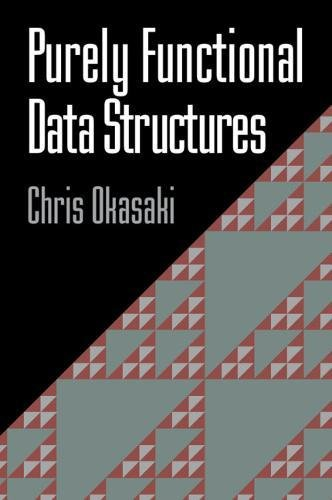
\includegraphics[scale=0.5]{okasaki_cover.jpg}
\end{subfigure}
\begin{subfigure}{.55\textwidth}
\begin{center}
  Подробнее в книге К.Окасаки \\"Чисто функциональные структуры данных" \\
  \vspace{6em}
    
  {\Huge Конец}
\end{center}
\end{subfigure}
\end{figure}
\end{frame}


\begin{frame}%[allowframebreaks]
\frametitle<presentation>{Ссылки}
\begin{thebibliography}{10}
\bibitem{paper}
  Книга "Чисто функциональные структуры данных"
 \newblock {\em Chris Okasaki}

\bibitem{leftist-ocaml}
  \href{http://typeocaml.com/2015/03/12/heap-leftist-tree/}{Heap -- Leftist Tree}
  
\bibitem{aa}
  \href{https://doi.org/10.1145/2857274.2884038}{Immutability changes everything}
  \newblock {\em Pat Helland  }
  
\bibitem{youtube}
  \href{https://www.youtube.com/watch?v=Wo0qiGPSV-s}{Immutable data structures for functional JS}
  \newblock {\em Anjana Vakil}
  
\end{thebibliography}
\end{frame}

\end{document}
